         \chapter{Classification of matter}\fancyfoot[LO,RE]{Chemistry: Matter and Materials}
    \setcounter{figure}{1}
    \setcounter{subfigure}{1}
%     \label{09a7a4809656be0b739ee130746cd803}
%          \section{Mixtures, compounds and elements}
%     \nopagebreak
    \label{m38708*cid1}
            \section{Materials}
            \nopagebreak
            \label{m38708} $ \hspace{-5pt}\begin{array}{cccccccccccc}   
\includegraphics[width=0.75cm]{col11305.imgs/summary_fullmarks.png} &   \end{array} $ \hspace{2 pt}\raisebox{-5 pt}{} {(section shortcode: P10011 )} \par 

            \label{m38708*id62175}All the objects that we see in the world around us, are made of \textbf{matter}. Matter makes up the air we breathe, the ground we walk on, the food we eat and the animals and plants that live around us. Even our own human bodies are made of matter!\par 
\begin{minipage}{.5\textwidth}
      \label{m38708*id62185}Different objects can be made of different types of \textbf{materials} (the matter from which objects are made). For example, a cupboard (an \textsl{object}) is made of wood, nails, hinges and knobs (the \textsl{materials}). The \textbf{properties} of the materials will affect the properties of the object. In the example of the cupboard, the strength of the wood and metals make the cupboard strong and durable. Electrical wires are made of metal (e.g. copper) because metals are a type of material that is able to conduct electricity. It is very important to understand the properties of materials, so that we can use them in our homes, in industry and in other applications. In this chapter, we will be looking at different types of materials and their properties.\par 
\end{minipage}
\begin{minipage}{.5\textwidth}
\begin{center}
 \includegraphics[width=.8
\textwidth]{photos/cupboardby-grongar-flickr.jpg}\par
\textit{Picture by grongar on Flickr.com}
\end{center}
\end{minipage} \\
\label{m38708*id0132}Some of the properties of matter that you should know are:
\label{m38708*lid825}\begin{itemize}[noitemsep]
  \item Materials can be \textbf{strong} and resist bending (e.g. bricks, rocks) or \textbf{weak} and bend easily (e.g. clothes)
  \item Materials that conduct heat (e.g. metals) are called \textbf{thermal conductors}. Materials that conduct electricity (e.g. copper wire) are \textbf{electrical conductors}.
  \item \textbf{Brittle} materials break easily (e.g. plastic). Materials that are \textbf{malleable} can be easily formed into different shapes (e.g. clay, dough). \textbf{Ductile} materials are able to be formed into long wires (e.g. copper).
  \item \textbf{Magnetic} materials have a magnetic field (e.g. iron).
  \item \textbf{Density} is the mass per unit volume. Examples include mud, concrete and stones.
  \item The \textbf{boiling and melting points} of substances tells us the temperature at which the substance will boil or melt. This helps us to classify substances as solids, liquids or gases at a specific temperature.\end{itemize}
\par 
      \label{m38708*id62556}The diagram below shows one way in which matter can be classified (grouped) according to its different properties. As you read further in this chapter, you will see that there are also other ways of classifying materials, for example according to whether or not they are good electrical conductors.\par 
    \setcounter{subfigure}{0}
	\begin{figure}[H] % horizontal\label{m38708*uid1}
    \begin{center}
    %\rule[.1in]{\figurerulewidth}{.005in} \\
     %   \label{m38708*uid1!!!underscore!!!media}\label{m38708*uid1!!!underscore!!!printimage}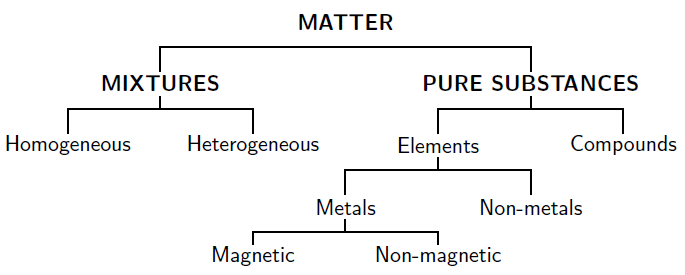
\includegraphics[width=300px]{col11305.imgs/m38708_CG10C1_001.png} % m38708;CG10C1\_001.png;;;6.0;8.5;
      %\vspace{2pt}
    %\vspace{\rubberspace}\par \begin{cnxcaption}
\begin{pspicture}(-6,0.5)(6,5)
%\psgrid[gridcolor=lightgray]
\rput(0,4.8){\textbf{MATTER}}
\psline(-3,4)(-3,4.4)(3,4.4)(3,4)
\rput(-3,3.8){\textbf{MIXTURES}}
\rput(3,3.8){\textbf{PURE SUBSTANCES}}
\psline(-3,3.4)(-3,3.6)
\psline(3,3.4)(3,3.6)
\psline(-4.5,3)(-4.5,3.4)(-1.5,3.4)(-1.5,3)
\psline(4.5,3)(4.5,3.4)(1.5,3.4)(1.5,3)
\rput(-4.5,2.8){Homogeneous}
\rput(-1.5,2.8){Heterogeneous}
\rput(4.5,2.8){Compounds}
\rput(1.5,2.8){Elements}
\psline(1.5,2.6)(1.5,2.4)
\psline(0,2.0)(0,2.4)(3,2.4)(3,2.0)
\rput(0,1.8){Metals}
\rput(3,1.8){Non-metals}
\psline(0,1.4)(0,1.6)
\psline(-1.5,1.2)(-1.5,1.4)(1.5,1.4)(1.5,1.2)
\rput(-1.5,1){Magnetic}
\rput(1.5,1){Non-magnetic}
%\psset{yunit=0.5}
\end{pspicture}

%	  \small \textbf{Figure 1.1: }The classification of matter
%	\end{cnxcaption}
%    \vspace{.1in}
 %   \rule[.1in]{\figurerulewidth}{.005in} \\
    \end{center}
\caption{The classification of matter}
\label{fig:c:ClassificationOfMatter}
 \end{figure}       
    \label{m38708*eip-344}\begin{activity}{What materials are products made of?}
{
\begin{minipage}{.5\textwidth}
This activity looks at the materials that make up food products. In groups of 3 or 4 look at the labels on food items. Make a list of the ingredients. Can you tell from the ingredients what the food is (i.e. spice, oil, sweets, etc.)? Food products are labelled to help you (the consumer) know what you are eating and to help you choose healthier alternatives. Some compounds, such as MSG and tartrazine are being removed from products due to being regarded as unsafe. Are there other ingredients in the products that are unsafe to eat? What preservatives and additives (e.g. tartrazine, MSG, colourants) are there? Are these preservatives and additives good for you? Are there natural (from plants) alternatives? What do different indigineous people groups use to flavour and preserve their food? 
\end{minipage}
\begin{minipage}{.5\textwidth}
 \begin{center}
 \includegraphics[width=.8\textwidth]{photos/food_labels.png}\par
\end{center}
\end{minipage}

 }  \end{activity}\par \label{m38708*cid2}
            \section{Mixtures}
            \nopagebreak
            \label{m38708*id62584}We see mixtures all the time in our everyday lives. A stew, for example, is a mixture of different foods such as meat and vegetables; sea water is a mixture of water, salt and other substances, and air is a mixture of gases such as carbon dioxide, oxygen and nitrogen.\par \pagebreak
\label{m38708*fhsst!!!underscore!!!id69}
\Definition{\label{id2405672}Mixture} {\label{m38708*meaningfhsst!!!underscore!!!id69}
      A \textbf{mixture} is a combination of two or more substances, where these substances are not bonded (or joined) to each other and no chemical reaction occurs. 
       } 
      \label{m38708*id62612}In a mixture, the substances that make up the mixture:\par 
      \label{m38708*id62615}\begin{itemize}[noitemsep]
            \label{m38708*uid2}\item \textbf{are not in a fixed ratio} \\
Imagine, for example, that you have 250 ml of water and you add sand to the water. It doesn't matter whether you add 20 g, 40 g, 100 g or any other mass of sand to the water; it will still be called a mixture of sand and water.
\label{m38708*uid3}\item \textbf{keep their physical properties} \\
In the example we used of the sand and water, neither of these substances has changed in any way when they are mixed together. The sand is still sand and the water is still water.
\label{m38708*uid4}\item \textbf{can be separated by mechanical means} \\
To separate something by 'mechanical means', means that there is no chemical process involved. In our sand and water example, it is possible to separate the mixture by simply pouring the water through a filter. Something \textsl{physical} is done to the mixture, rather than something \textsl{chemical}.
\end{itemize}
      \label{m38708*id62700}We can group mixtures further by dividing them into those that are heterogeneous and those that are homogeneous.\par 

      \label{m38708*uid5}
            \subsection*{Heterogeneous mixtures}
            \nopagebreak
        \label{m38708*id62715}A \textbf{heterogeneous} mixture does not have a definite composition. Cereal in milk is an example of a heterogeneous mixture. Soil is another example. Soil has pebbles, plant matter and sand in it. Although you may add one substance to the other, they will stay separate in the mixture. We say that these heterogeneous mixtures are \textsl{non-uniform}, in other words they are not exactly the same throughout.\par 
\begin{minipage}{.5\textwidth}
\begin{center}
 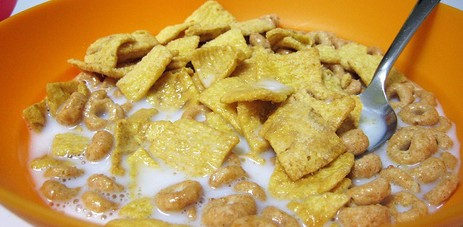
\includegraphics[width=.8\textwidth]{photos/mixtureby-dougww-flickr.jpg}\par
\textit{Picture by dougww on Flickr.com}
\end{center}
\end{minipage}
\begin{minipage}{.5\textwidth}
\begin{figure}[H]
\label{fig:heterogeneousmixture}
\begin{center}
 \begin{pspicture}(0,-1)(11,4.7)
\SpecialCoor
\psframe[fillstyle=crosshatch*,fillcolor=white,hatchcolor=lightgray,hatchwidth=1.2pt,hatchsep=1.8pt,hatchangle=0](0,0)(4,4)
\pscircle[fillcolor=lightgray,fillstyle=solid](0.5,0.5){0.2}
\pscircle[fillcolor=white,fillstyle=solid](1,1.2){0.1}
\pscircle[fillcolor=lightgray,fillstyle=solid](2.1,1){0.2}
\pscircle[fillcolor=white,fillstyle=solid](2.3,0.4){0.1}
\pscircle[fillcolor=lightgray,fillstyle=solid](3.5,1){0.2}
\pscircle[fillcolor=white,fillstyle=solid](0.5,1.6){0.1}
\pscircle[fillcolor=white,fillstyle=solid](1,2){0.1}
\pscircle[fillcolor=white,fillstyle=solid](1.8,1.5){0.1}
\pscircle[fillcolor=lightgray,fillstyle=solid](2,2){0.2}
\pscircle[fillcolor=lightgray,fillstyle=solid](0.5,2.7){0.2}
\pscircle[fillcolor=lightgray,fillstyle=solid](2.3,2.5){0.2}
\pscircle[fillcolor=white,fillstyle=solid](2.5,2.8){0.1}
\pscircle[fillcolor=white,fillstyle=solid](3,3){0.1}
\pscircle[fillcolor=white,fillstyle=solid](3.5,2.4){0.1}
\pscircle[fillcolor=white,fillstyle=solid](0.5,3.5){0.1}
\pscircle[fillcolor=white,fillstyle=solid](2,3.4){0.1}
\pscircle[fillcolor=lightgray,fillstyle=solid](3.5,3.5){0.2}
\pscircle[fillcolor=lightgray,fillstyle=solid](1.7,3.1){0.2}
\pscircle[fillcolor=white,fillstyle=solid](3,3){0.1}
\end{pspicture}
\end{center}
\caption{A submicroscopic representation of a heterogeneous mixture. The gray circles are one substance (e.g. one cereal) and the white circles are another substance (e.g. another cereal). The background is the milk.}
\end{figure}
\end{minipage}


\label{m38708*fhsst!!!underscore!!!id89}\Definition{\label{id2405839} { Heterogeneous mixture }} 
{ \label{m38708*meaningfhsst!!!underscore!!!id89}
        A heterogeneous mixture is one that consists of two or more substances and is non-uniform and the different components of the mixture can be seen.
         } 
Heterogeneous mixtures can be further subdivided according to whether it is two liquids mixed, a solid and a liquid or a liquid and a gas or even a gas and a solid. These mixtures are given special names which you can see in table below. \par
\begin{table}[h!]
 \begin{center}
  \begin{tabular}{|l|l|l|}\hline
   \textbf{Phases of matter} & \textbf{Name of mixture} & \textbf{Example} \\ \hline
   liquid-liquid & Emulsion & milk \\ \hline
   solid-liquid & Suspension & muddy water \\ \hline
   liquid-gas & Aerosol & fizzy drinks \\ \hline
   gas-solid & Foam & smoke \\ \hline
  \end{tabular}

 \end{center}
\caption{Examples of different heterogeneous mixtures}
\label{tab:mixtures}
\end{table}
\\
      \label{m38708*uid6}
            \subsection*{Homogeneous mixtures}
            \nopagebreak
        \label{m38708*id62762}A \textbf{homogeneous} mixture has a definite composition, and specific properties. In a homogeneous mixture, the different parts cannot be seen. A solution of salt dissolved in water is an example of a homogeneous mixture. When the salt dissolves, it spreads evenly through the water so that all parts of the solution are the same, and you can no longer see the salt as being separate from the water. Think also of coffee without milk. The air we breathe is another example of a homogeneous mixture since it is made up of different gases which are in a constant ratio, and which can't be visually distinguished from each other (i.e. you can't see the different components).\par 
\begin{minipage}{.5\textwidth}
\begin{center}
 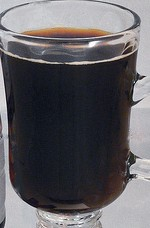
\includegraphics[width=.3\textwidth]{photos/mix2by-javcon117-flickr.jpg}\par
\textit{Picture by javcon117 on Flickr.com}
\end{center}
\end{minipage}
\begin{minipage}{.5\textwidth}
\begin{center}
 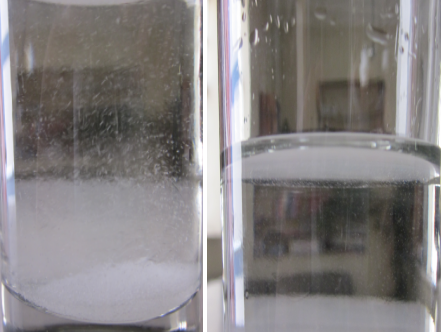
\includegraphics[width=.5\textwidth]{photos/saltwater.png}\par
\end{center}
\end{minipage}
\label{m38708*fhsst!!!underscore!!!id96}\Definition{   \label{id2405912}Homogeneous mixture} { \label{m38708*meaningfhsst!!!underscore!!!id96}
        A homogeneous mixture is one that is uniform, and where the different components of the mixture cannot be seen. 
         } 
        \label{m38708*id62795}An \textbf{alloy} is a homogeneous mixture of two or more elements, at least one of which is a metal, where the resulting material has metallic properties. Alloys are usually made to improve the properties of the elements that make them up. For example steel is much stronger than iron (which is the main component of steel). Steel is a mixture (alloy) of mainly iron with carbon (to make it harder), manganese (to make it strong) and chromium (to prevent rusting).\par 
\label{m38708*eip-479}
%\vspace{.5cm} 
%      \noindent
%      \hspace*{-30pt}
\includegraphics[width=0.5in]{col11305.imgs/pspencil2.png}   \raisebox{25mm}{   
%      \begin{mdframed}[linewidth=4, leftmargin=40, rightmargin=40]  
      \begin{wex}{Mixtures}
%\label{m38708*eip-277}
%\label{m38708*eip-353}
{For each of the following mixtures state whether it is a homogenous or a heterogenous mixture:
\label{m38708*eip-id1167649056231}\begin{enumerate}[noitemsep, label=\textbf{\alph*}. ] 
            \leftskip=20pt\rightskip=\leftskip\item sugar dissolved in water
\item flour and iron filings (small pieces of iron)
\item flour and baking powder\item smarties, jelly tots and peppermints\end{enumerate} }
%  \par 
%\vspace{5pt}
%\label{m38708*eip-602}\noindent\textbf{Solution to Exercise }
%\label{m38708*eip-id7325184}
{\westep{Look at the definition}
We first look at the definition of a heterogeneous and homogeneous mixture.
\westep{Decide whether or not you can see the components}
\begin{enumerate}[noitemsep, label=\textbf{\alph*}. ] 
 %           \leftskip=20pt\rightskip=\leftskip
\item We cannot see the sugar in the water.
\item We are able to make out the pieces of iron in the flour.
\item There is no way to distinguish between the flour and the baking powder.
\item We can clearly see each of the components that make up the mixture. \end{enumerate}
\westep{Decide whether or not the components are mixed uniformly}
\begin{enumerate}[noitemsep, label=\textbf{\alph*}. ] 
 %           \leftskip=20pt\rightskip=\leftskip
\item The two components are mixed uniformly.
\item In this mixture there may be places where there are a lot of iron filings and places where there is more flour, so it is not uniformly mixed.
\item The two components of the mixture are uniformly mixed.
\item The three components of the mixture are not evenly distributed.\end{enumerate}
\westep{Give the final answer}
\begin{enumerate}[noitemsep, label=\textbf{\alph*}. ] 
 %           \leftskip=20pt\rightskip=\leftskip
\item Homogenous mixture.
\item Heterogenous mixture.
\item Homogenous mixture.
\item Heterogenous mixture.\end{enumerate}}
    \end{wex}
%    \end{mdframed}
 
 %   \noindent
  \label{m38708*eip-478}\begin{activity}{Classifying materials}
{\begin{minipage}{.5\textwidth}
Look around you at the buildings and other structures. Make a list of all the different materials that you see around you. Try to work out why a particular material was used. Can you classify all the different materials used according to their properties? On your way to school or at home or in the shops, look at the different materials that are used. Why are these materials chosen over other materials?\par \label{m38708*eip-894}
\end{minipage}
\begin{minipage}{.5\textwidth}
\begin{center}
 \includegraphics[width=.8\textwidth]{photos/materials.png}\par
\end{center}
\end{minipage}
}
\end{activity}
\begin{activity}{Making mixtures}
{Make mixtures of sand and water, potassium dichromate and water, iodine and ethanol, iodine and water. Classify these as heterogeneous or homogeneous. Try to make mixtures using other substances. Are the mixtures that you have made heterogeneous or homogeneous? Give reasons for your choice. \par}
\end{activity}
\label{m38708*secfhsst!!!underscore!!!id169}
\begin{exercises}{Mixtures}
{Complete the following table: \par
%\nopagebreak
\begin{tabular}{|l|l|l|l|}\hline
\textbf{Substance} & \textbf{Element or} & \textbf{Heterogeneous} & \textbf{Homogeneous} \\ 
 & \textbf{mixture} & \textbf{mixture} & \textbf{mixture} \\ \hline
tap water & & & \\ \hline
brass (an alloy of copper and zinc) & & & \\ \hline
concrete & & & \\ \hline
aluminium foil (tinfoil) & & & \\ \hline
Coca cola & & & \\ \hline
distilled water & & & \\ \hline
\end{tabular}
    \label{m38708*cid3}
\par \raisebox{-5 pt}{
\includegraphics[width=0.5cm]{col11305.imgs/summary_www.png}} Find the answers with the shortcodes:
 \par \begin{tabular}[h]{cccccc}
 (1.) llm  & \end{tabular} }
\end{exercises}
            \section{Pure Substances: Elements and Compounds}
            \nopagebreak
      \label{m38708*id63273}Any material that is not a mixture, is called a \textbf{pure substance}. Pure substances include \textbf{elements} and \textbf{compounds}. It is much more difficult to break down pure substances into their parts, and complex chemical methods are needed to do this.\par 
      \label{m38708*eip-862}One way to determine if a substance is pure is to look at its melting or boiling point. Pure substances will have a sharply defined melting or boiling point (i.e. the melting or boiling point will be a single temperature rather than a range of temperatures.) Impure substances have a temperature range over which they melt or boil. We can also use chromatography to determine if a substance is pure or not. Chromatography is the process of separating substances into their individual components. If a substance is pure then chromatography will only produce one substance at the end of the process. If a substance is impure then several substances will be seen at the end of the process. \par \label{m38708*eip-122}
%NTS: DIAGRAM needed for the following experiment
\begin{activity}{Recommended practical activity: Smartie chromatography}{You will need filter paper (or chromatography paper), some smarties in different colours, water and an eye dropper. \newline
\begin{figure}[h]
\label{fig:smartiechromatography}
\begin{center}
 \begin{pspicture}(0,-1)(11,4.7)
\SpecialCoor
%\psframe(0,0)(5,5)
\pscircle[fillcolor=white,fillstyle=solid](2,2){1}
\pscircle[fillcolor=lightgray,fillstyle=solid](2,2){0.3}
\psline[linewidth=0.04]{->}(2,2)(4.5,2)
\uput[r](4.5,2){\large{smartie}}
\psline[linewidth=0.04]{->}(2.5,2.5)(4.5,2.5)
\uput[r](4.5,2.5){\large{filter paper}}
\end{pspicture}
\end{center}
\end{figure}\newline
Place a smartie in the center of a piece of filter paper. Carefully drop a few drops of water onto the smartie. You should see rings of different colour forming around the smartie. Each colour is one of the individual colours that are used to make up the colour of the smartie.}
\end{activity}
\par \label{m38708*eip-392}
%\begin{tabular}{cc}
%	\hspace*{-50pt}\raisebox{-8 mm}{\hspace{-0.2in}
\includegraphics[width=0.5in]{col11305.imgs/pstip2.png} } & 
%	\begin{minipage}{0.85\textwidth}
	\Tip
      {For the above activity you can use ordinary filter paper (that is used in coffee filters) from your local store.}
%	\end{minipage}
%	\end{tabular}
	\par
      \label{m38708*uid25}
            \subsection*{Elements}
            \nopagebreak
        \label{m38708*id63302}An \textbf{element} is a chemical substance that can't be divided or changed into other chemical substances by any ordinary chemical means. The smallest unit of an element is the \textbf{atom}.\par 
\label{m38708*fhsst!!!underscore!!!id193}
\Definition{   \label{id2406278} Element } 
{ \label{m38708*meaningfhsst!!!underscore!!!id193}
An element is a substance that cannot be broken down into other substances through chemical means.} 
        \label{m38708*id63334}There are 112 officially named elements and about 118 known elements. Most of these are natural, but some are man-made. The elements we know are represented in the \textbf{Periodic Table of the Elements}, where each element is abbreviated to a \textbf{chemical symbol}. Examples of elements are magnesium ($\mathrm{Mg}$), hydrogen ($\mathrm{H}$), oxygen ($\mathrm{O}$) and carbon ($\mathrm{C}$). On the Periodic Table you will notice that some of the abbreviations do not seem to match the elements they represent. The element iron, for example, has the chemical formula $\mathrm{Fe}$. This is because the elements were originally given Latin names. Iron has the abbreviation $\mathrm{Fe}$ because its Latin name is 'ferrum'. In the same way, sodium's Latin name is 'natrium' ($\mathrm{Na}$) and gold's is 'aurum' ($\mathrm{Au}$).\par \label{m38708*eip-775}
The following table gives the first 20 elements and some of the common transition metals.\par
\begin{table}[h!]
\label{tab:elements}
\begin{center}
\begin{tabular}{|l|l|l|l|}\hline
\textbf{Element name} & \textbf{Element symbol} & \textbf{Element name} & \textbf{Element symbol} \\ \hline
Hydrogen & $\mathrm{H}$ & Phosphorus & $\mathrm{P}$  \\ \hline
Helium & $\mathrm{He}$ & Sulphur & $\mathrm{S}$ \\ \hline
Lithium & $\mathrm{Li}$ & Chlorine & $\mathrm{Cl}$ \\ \hline
Beryllium & $\mathrm{Be}$ & Argon & $\mathrm{Ar}$ \\ \hline 
Boron & $\mathrm{B}$ & Potassium & $\mathrm{K}$ \\ \hline
Carbon & $\mathrm{C}$ & Calcium & $\mathrm{Ca}$ \\ \hline 
Nitrogen & $\mathrm{N}$ & Iron & $\mathrm{Fe}$ \\ \hline
Oxygen & $\mathrm{O}$ & Nickel & $\mathrm{Ni}$ \\ \hline 
Fluorine & $\mathrm{F}$ & Copper & $\mathrm{Cu}$ \\ \hline
Neon & $\mathrm{Ne}$  & Zinc & $\mathrm{Zn}$ \\ \hline
Sodium & $\mathrm{Na}$  & Silver & $\mathrm{Ag}$ \\ \hline
Magnesium & $\mathrm{Mg}$  & Platinum & $\mathrm{Pt}$ \\ \hline
Aluminium & $\mathrm{Al}$ & Gold & $\mathrm{Au}$ \\ \hline
Silicon & $\mathrm{Si}$ & Mercury & $\mathrm{Hg}$  \\ \hline
\end{tabular}
\end{center}
\caption{List of the first 20 elements and some common transition metals}
\end{table}
\par
%\begin{tabular}{cc}
%	\hspace*{-50pt}\raisebox{-8 mm}{\hspace{-0.2in}
\includegraphics[width=0.75in]{col11305.imgs/psfact2.png} } & 
%	\begin{minipage}{0.85\textwidth}
%	\begin{note}
      \IFact{Recently it was agreed that two more elements would be added to the list of officially named elements. These are elements number 114 and 116. The proposed name for element 114 is flerovium and for element 116 it is moscovium. This brings the total number of officially named elements to 114.}
%	\end{note}
%	\end{minipage}
%	\end{tabular}
	\par
      \label{m38708*uid26}
            \subsection*{Compounds}
            \nopagebreak
        \label{m38708*id63363}A \textbf{compound} is a chemical substance that forms when two or more different elements combine in a fixed ratio. Water ($\mathrm{H}{}_{2}\mathrm{O}$), for example, is a compound that is made up of two hydrogen atoms for every one oxygen atom. Sodium chloride ($\mathrm{NaCl}$) is a compound made up of one sodium atom for every chlorine atom. An important characteristic of a compound is that it has a \textbf{chemical formula}, which describes the ratio in which the atoms of each element in the compound occur.\par 
\label{m38708*fhsst!!!underscore!!!id201}
%\begin{definition}
%	  \begin{tabular*}{15 cm}{m{15 mm}m{}}
%	\hspace*{-50pt}  
\includegraphics[width=0.5in]{col11305.imgs/psflag2.png}   & 
\Definition{\label{id2406453} Compound } { \label{m38708*meaningfhsst!!!underscore!!!id201}
        A substance made up of two or more different elements that are joined together in a fixed ratio.
         } 
%       \end{tabular*}
%       \end{definition}
        \label{m38708*id63410} Figure \ref{fig:classification:mixture and compound} might help you to understand the difference between the terms \textbf{element}, \textsbf{mixture} and \textsbf{compound}. Iron ($\mathrm{Fe}$) and sulphur ($\mathrm{S}$) are two elements. When they are added together, they form a \textsl{mixture} of iron and sulphur. The iron and sulphur are not joined together. However, if the mixture is heated, a new \textbf{compound} is formed, which is called iron sulphide ($\mathrm{FeS}$). In this compound, the iron and sulphur are joined to each other in a ratio of 1:1. In other words, one atom of iron is joined to one atom of sulphur in the compound iron sulphide.\par 
    \setcounter{subfigure}{0}
	\begin{figure}[H] % horizontal\label{m38708*uid27}
    \begin{center}
 \begin{pspicture}(0,-1)(11,4.7)
\SpecialCoor
%\psgrid[gridcolor=lightgray]
\def\fe{\pscircle[fillcolor=lightgray,fillstyle=solid](0,0){0.4}\rput(0,0){Fe}}
\def\s{\pscircle[fillcolor=white,fillstyle=solid](0,0){0.2}\rput(0,0){S}}
\def\fes{\fe \rput(0.6,0){\s}} 

\psframe(0,0)(4,4)
\rput(1.5,2){\s}
\rput{30}(3,1){\rput(1,1){\fe}\rput(1.5,2){\s}}
\rput{65}(1.55,1.33){\rput(1,1){\fe}\rput(1.5,2){\s}}
\rput{265}(2,3){\rput(-0.1,0.4){\fe}\rput(1.5,1.6){\s}}
\rput(2,0.6){\s}
\rput(1,1){\fe}
\rput(3,0.7){\fe}
\rput(2.4,2){\fe}
\rput(1.4,3.6){\s}
\psline(3.4,0.6)(4.2,0.6)
\uput[r](4.2,0.6){\parbox{1.5cm}{An atom of the element iron (Fe)}}

\psline(3.5,3.5)(4.2,3.5)
\uput[r](4.2,3.5){\parbox{1.5cm}{An atom of the element sulfur (S)}}
\rput(2,-0.5){\parbox{4cm}{A mixture of iron and sulfur}}

\rput(7,0){
\psframe(0,0)(4,4)
\rput{30}(1,2){\fes}
\rput{45}(1,1){\fes}
\rput{90}(3,0.7){\fes}
\rput{245}(1,3.5){\fes}
\rput{190}(3,3.2){\fes}
\rput{60}(2.4,2){\fes}
\rput(2,-0.5){\parbox{4cm}{The compound iron sulfide (FeS)}}
}

\end{pspicture}
\caption{Understanding the difference between a mixture and a compound}
\label{fig:classification:mixture and compound}
    \end{center}
 \end{figure}       
\label{m38708*eip-487} Figure \ref{fig:classification:mixture and compound} shows the submicroscopic representation of mixtures and compounds. In a submicroscopic representation we use circles to represent different elements. To show a compound, we draw several circles joined together. Mixtures are simply shown as two or more individual elements in the same box. The circles are not joined for a mixture.\par 
\label{m38708*id0124}We can also use symbols to represent elements, mixtures and compounds. The symbols for the elements are all found on the periodic table. Compounds are shown as two or more element names written right next to each other. Subscripts may be used to show that there is more than one atom of a particular element. (e.g. $\mathrm{H}{}_{2}\mathrm{O}$ or $\mathrm{NH}_{3}$). Mixtures are written as: a mixture of element (or compound) A and element (or compound) B. (e.g. a mixture of $\mathrm{Fe}$ and $\mathrm{S}$).\par 
\label{m38708*eip-595}One way to think of mixtures and compounds is to think of buildings. The building is a mixture of different building materials (e.g. glass, bricks, cement, etc.). The building materials are all compounds. You can also think of the elements as Lego blocks. Each Lego block can be added to other Lego building blocks to make new structures, in the same way that elements can combine to make compounds. \par \label{m38708*eip-524}\vspace{.5cm} 
%      \noindent
%      \hspace*{-30pt}
\includegraphics[width=0.5in]{col11305.imgs/pspencil2.png}   \raisebox{25mm}{   
%      \begin{mdframed}[linewidth=4, leftmargin=40, rightmargin=40]  
      \begin{wex}
%    \noindent\textbf
{Mixtures and pure substances}
%\label{m38708*eip-259}
 % \label{m38708*eip-457}
{For each of the following substances state whether it is a pure substance or a mixture. If it is a mixture, is it homogenous or heterogenous? If it is a pure substance is it an element or a compound? 
\label{m38708*eip-id1167351497334}\begin{enumerate}[noitemsep, label=\textbf{\alph*}. ] 
   %         \leftskip=20pt\rightskip=\leftskip
\item Blood
\item Argon
\item Silicon dioxide (${\mathrm{SiO}}_{2}$)
\item Sand and stones
\end{enumerate}
  \par }
%\vspace{5pt}
%\label{m38708*eip-62}\noindent\textbf{Solution to Exercise }
%\label{m38708*eip-id1167366034146}
{\westep{Look at the definitions}
 
 %           \leftskip=20pt\rightskip=\leftskip
\begin{enumerate}
[noitemsep, label=\textbf{\alph*}. ]
\item Blood is a mixture since it is made up of many different compounds and substances. Blood is a homogenous mixture since you cannot see the individual components and the components are uniformly distributed.
\item Argon is a pure substance. Argon is an element since we can find it on the periodic table.
\item Silicon dioxide is a pure substance. It is a compound since it is made of the elements silicon and oxygen joined in a fixed ratio.
\item Sand and stones form a mixture. There are two distinct compounds. It is a heterogenous mixture since the particles are not uniformly distributed and we can see the individual pieces.
\end{enumerate}}
    \end{wex}
%    \end{mdframed}
%    }
%    \noindent
\vspace{-1cm}
  \label{m38708*eip-326}
\begin{activity}{Using models to represent substances}{Use coloured balls and sticks to represent elements and compounds. Some examples that you can try to build are:
\label{m38708*eip-id1166921187210}
\begin{itemize}[noitemsep]
    \item Hydrogen
    \item Oxygen
    \item Nitrogen
    \item Neon
    \item Sodium chloride (salt, $\mathrm{NaCl}$)
    \item Potassium permanganate (${\mathrm{KMnO}}_{4}$)
    \item Water (${\mathrm{H}}_{2}\mathrm{O}$)
    \item Iron sulphide ($\mathrm{FeS}$)
\end{itemize}
Think about the way that we represent substances submicroscopically. Draw these submicroscopic representations for each of the above examples. Would you use just one ball to represent an element or many? Why? }
\end{activity}
\par \label{m38708*secfhsst!!!underscore!!!id212}
            \begin{exercises}{Elements, mixtures and compounds}{
            \nopagebreak
            \label{m38708*id63472}
 \begin{enumerate}[noitemsep, label=\textbf{\arabic*}. ] 
            \label{m38708*uid28}
    \item In the following table, tick whether each of the substances listed is a \textsl{mixture} or a \textsl{pure substance}. If it is a mixture, also say whether it is a homogeneous or heterogeneous mixture.
    % \textbf{m38708*id63499}\par
          \begin{table}[H]
    % \begin{table}[H]
    % \\ 'id2876023' '1'
        \begin{center}
      \label{m38708*id63499}
    \noindent
    \tabletail{%
        \hline
        \multicolumn{3}{|p{\mytableboxwidth}|}{\raggedleft \small \sl continued on next page}\\
        \hline
      }
      \tablelasttail{}
      \begin{xtabular}[t]{|l|l|l|}\hline
        \textbf{Substance} &
        \textbf{Mixture or pure} &
        \textbf{Homogeneous or heterogeneous mixture}% make-rowspan-placeholders
     \tabularnewline\cline{1-1}\cline{2-2}\cline{3-3}
      %--------------------------------------------------------------------
        fizzy colddrink &
         &
        % make-rowspan-placeholders
     \tabularnewline\cline{1-1}\cline{2-2}\cline{3-3}
      %--------------------------------------------------------------------
        steel &
         &
        % make-rowspan-placeholders
     \tabularnewline\cline{1-1}\cline{2-2}\cline{3-3}
      %--------------------------------------------------------------------
        oxygen &
         &
        % make-rowspan-placeholders
     \tabularnewline\cline{1-1}\cline{2-2}\cline{3-3}
      %--------------------------------------------------------------------
        iron filings &
         &
        % make-rowspan-placeholders
     \tabularnewline\cline{1-1}\cline{2-2}\cline{3-3}
      %--------------------------------------------------------------------
        smoke &
         &
        % make-rowspan-placeholders
     \tabularnewline\cline{1-1}\cline{2-2}\cline{3-3}
      %--------------------------------------------------------------------
        limestone (${\mathrm{CaCO}}_{3}$) &
         &
        % make-rowspan-placeholders
     \tabularnewline\cline{1-1}\cline{2-2}\cline{3-3}
      %--------------------------------------------------------------------
    \end{xtabular}
      \end{center}
%    \begin{center}{\small\bfseries Table 1.1}\end{center}
%    \begin{caption}{\small\bfseries Table 1.1}\end{caption}
\end{table}
    \par
\label{m38708*uid29}\item In each of the following cases, say whether the substance is an element, a mixture or a compound.
\label{m38708*id63912}\begin{enumerate}[noitemsep, label=\textbf{\alph*}. ] 
            \label{m38708*uid30}\item $\mathrm{Cu}$
\label{m38708*uid31}\item iron and sulphur
\label{m38708*uid32}\item $\mathrm{Al}$
\label{m38708*uid33}\item $\mathrm{H}{}_{2}\mathrm{SO}{}_{4}$\label{m38708*uid34}\item $\mathrm{SO}{}_{3}$\end{enumerate}
                \end{enumerate}
    \label{m38708*cid4}
\par \raisebox{-5 pt}{
\includegraphics[width=0.5cm]{col11305.imgs/summary_www.png}} Find the answers with the shortcodes:
 \par \begin{tabular}[h]{cccccc}
 (1.) lly  &  (2.) llV  & \end{tabular}}
\end{exercises}
%NTS DIAGRAM is needed here and some more examples in the above exercises
            \section{Giving names and formulae to substances}
            \nopagebreak
      \label{m38708*eip-379}Think about what you call your friends. Some of your friends might have full names (long names) and a nickname (short name). These are the words we use to tell others who or what we are referring to. Their full name is like the substances name and their nickname is like the substances formulae. Without these names your friends would have no idea which of them you are referring to. Chemical substances have names, just like people have names. This helps scientists to communicate efficiently.     \par \label{m38708*id64028}It is easy to describe elements and mixtures. We simply use the names that we find on the periodic table for elements and we use words to describe mixtures. But how are compounds named? In the example of iron sulphide that was used earlier, the compound name is a combination of the names of the elements but slightly changed. \par 
      \label{m38708*id64033}The following are some guidelines for naming compounds:\par 
      \label{m38708*id64037}\begin{enumerate}[noitemsep, label=\textbf{\arabic*}. ] 
            \label{m38708*uid35}\item The compound name will always include the \textbf{names of the elements} that are part of it.
\label{m38708*id64059}\begin{itemize}[noitemsep]
            \label{m38708*uid36}\item A compound of \textbf{iron} ($\mathrm{Fe}$) and \textsl{sulphur} ($\mathrm{S}$) is \textbf{iron}\hspace{1ex}\textsl{sulph}ide ($\mathrm{FeS}$)
\label{m38708*uid37}\item A compound of \textbf{potassium} ($\mathrm{K}$) and \textsl{bromine} ($\mathrm{Br}$) is \textbf{potassium}\hspace{1ex}\textsl{brom}ide ($\mathrm{KBr}$)
\label{m38708*uid38}\item A compound of \textbf{sodium} ($\mathrm{Na}$) and \textsl{chlorine} ($\mathrm{Cl}$) is \textbf{sodium}\hspace{1ex}\textsl{chlor}ide ($\mathrm{NaCl}$)
\end{itemize}
        \label{m38708*uid39}\item In a compound, the element that is on the left of the Periodic Table, is used \textsl{first} when naming the compound. In the example of $\mathrm{NaCl}$, sodium is a group 1 element on the left hand side of the table, while chlorine is in group 7 on the right of the table. Sodium therefore comes first in the compound name. The same is true for $\mathrm{FeS}$ and $\mathrm{KBr}$.
\label{m38708*uid40}\item The \textbf{symbols} of the elements can be used to represent compounds e.g. $\mathrm{FeS}$, $\mathrm{NaCl}$, $\mathrm{KBr}$ and $\mathrm{H}{}_{2}\mathrm{O}$. These are called \textbf{chemical formulae}. In the first three examples, the ratio of the elements in each compound is 1:1. So, for $\mathrm{FeS}$, there is one atom of iron for every atom of sulphur in the compound. In the last example ($\mathrm{H}{}_{2}\mathrm{O}$) there are two atoms of hydrogen for every atom of oxygen in the compound.
\label{m38708*uid41}\item A compound may contain \textbf{compound ions}. An ion is an atom (or group of atoms) that has lost (positive ion) or gained (negative ion) electrons. Some of the more common compound ions and their formulae are given in table \ref{tab:cations} and in table \ref{tab:anions}.\\

    % \textbf{m38708*id64235}\par
    %      \begin{table}[H]
    % \begin{table}[H]
    % \\ 'id2876536' '1'
      
\begin{table}
\begin{center}
\label{tab:cations}
\begin{tabular}{|l|c|l|c|l|c|l|c|} \hline
\textbf{Compound ion} & \textbf{Formula} & \textbf{Compound ion} & \textbf{Formula} & \textbf{Compound ion} & \textbf{Formula}  \\ \hline
Hydrogen       & $\mathrm{H}^{+}$   & Lithium        & $\mathrm{Li}^{+}$     & Sodium          & $\mathrm{Na}^{+}$  \\ \hline
Potassium      & $\mathrm{K}^{+}$   & Silver         & $\mathrm{Ag}^{+}$     & Mercury (I)     & $\mathrm{Hg}^{+}$  \\ \hline
Copper (I)     & $\mathrm{Cu}^{+}$  & Ammonium       & $\mathrm{NH}_{4}^{+}$ & Beryllium       & $\mathrm{Be}^{2+}$ \\ \hline
Magnesium      & $\mathrm{Mg}^{2+}$ & Calcium        & $\mathrm{Ca}^{2+}$    & Barium          & $\mathrm{Ba}^{2+}$ \\ \hline
Tin (II)       & $\mathrm{Sn}^{2+}$ & Lead (II)      & $\mathrm{Pb}^{2+}$    & Chromium (II)   & $\mathrm{Cr}^{2+}$ \\ \hline
Manganese (II) & $\mathrm{Mn}^{2+}$ & Iron (II)      & $\mathrm{Fe}^{2+}$    & Cobalt (II)     & $\mathrm{Co}^{2+}$ \\ \hline
Nickel         & $\mathrm{Ni}^{2+}$ & Copper (II)    & $\mathrm{Cu}^{2+}$    & Zinc            & $\mathrm{Zn}^{2+}$ \\ \hline
Aluminium      & $\mathrm{Al}^{3+}$ & Chromium (III) & $\mathrm{Cr}^{3+}$    & Iron (III)      & $\mathrm{Fe}^{3+}$ \\ \hline
Cobalt (III)   & $\mathrm{Co}^{3}$  & Chromium (VI)  & $\mathrm{Cr}^{6+}$    & Manganese (VII) & $\mathrm{Mn}^{7+}$ \\ \hline

\end{tabular}

 \end{center}
\caption{Table of cations}
\label{tab:cations}
\end{table}

\begin{table}
\begin{center}
\label{tab:anions}
\begin{tabular}{|l|c|l|c|l|c|l|c|} \hline
\textbf{Compound ion} & \textbf{Formula}            & \textbf{Compound ion} & \textbf{Formula} \\ \hline
Fluoride             & $\mathrm{F}^{-}$             & Oxide              & $\mathrm{O}^{2-}$ \\ \hline
Chloride             & $\mathrm{Cl}^{-}$            & Peroxide           & $\mathrm{O}_{2}^{2-}$ \\ \hline
Bromide              & $\mathrm{Br}^{-}$            & Carbonate          & $\mathrm{CO}_{3}^{2-}$ \\ \hline
Iodide               & $\mathrm{I}^{-}$             & Sulphide           & $\mathrm{S}^{2-}$ \\ \hline
Hydroxide            & $\mathrm{OH}^{-}$            & Sulphite           & $\mathrm{SO}_{3}^{2-}$ \\ \hline
Nitrite              & $\mathrm{NO}_{2}^{-}$        & Sulphate           & $\mathrm{SO}_{4}^{2-}$ \\ \hline
Nitrate              & $\mathrm{NO}_{3}^{-}$        & Thiosulphate       & $\mathrm{S}_{2}{\mathrm{O}}_{3}^{2-}$ \\ \hline
Hydrogen carbonate   & $\mathrm{HCO}_{3}^{-}$       & Chromate           & $\mathrm{CrO}_{4}^{2-}$ \\ \hline
Hydrogen sulphite    & $\mathrm{HSO}_{3}^{-}$       & Dichromate         & $\mathrm{Cr}_{2}{\mathrm{O}}_{7}^{2-}$ \\ \hline
Hydrogen carbonate   & $\mathrm{HSO}_{4}^{-}$       & Manganate          & $\mathrm{MnO}_{4}^{2-}$ \\ \hline
Dihydrogen phosphate & $\mathrm{H}_{2}{\mathrm{PO}}_{4}^{-}$ & Oxalate   & $\mathrm{(COO)}_{2}^{2-}/{\mathrm{C}}_{2}{\mathrm{O}}_{4}^{2-}$ \\ \hline
Hypochlorite         & $\mathrm{ClO}^{-}$           & Hydrogen phosphate & $\mathrm{HPO}_{4}^{2-}$ \\ \hline
Chlorate             & $\mathrm{ClO}_{3}^{-}$       & Nitride            & $\mathrm{N}^{3-}$ \\ \hline
Permanganate         & $\mathrm{MnO}_{4}^{-}$       & Phosphate          & $\mathrm{PO}_{4}^{3-}$ \\ \hline
Acetate Ethanoate    & $\mathrm{CH}_{3}{\mathrm{COO}}^{-}$   & Phosphide          & $\mathrm{P}^{3-}$ \\ \hline
\end{tabular}

 \end{center}
\caption{Table of anions}
\label{tab:anions}
\end{table}

    \par
  \label{m38708*uid42}\item When there are only two elements in the compound, the compound is often given a \textbf{suffix} (ending) of -ide. You would have seen this in some of the examples we have used so far. For compound ions, when a non-metal is combined with oxygen to form a negative ion (anion) which then combines with a positive ion (cation) from hydrogen or a metal, then the suffix of the name will be ...ate or ...ite. $\mathrm{NO}_{3}^{-}$ for example, is a negative ion, which may combine with a cation such as hydrogen ($\mathrm{HNO}{}_{3}$) or a metal like potassium (KNO$_\text{3}$). The $\mathrm{NO}_{3}^{-}$ anion has the name nitr\textbf{ate}. $\mathrm{SO}_{3}^{2-}$ in a formula is sulph\textbf{ite}, e.g. sodium sulphite ($\mathrm{Na}{}_{2}\mathrm{SO}{}_{3}$).\newline
     $\mathrm{SO}_{4}^{2-}$ is sulph\textbf{ate} and $\mathrm{PO}_{4}^{3-}$ is phosph\textbf{ate}.
\label{m38708*uid43}\item \textbf{Prefixes} can be used to describe the ratio of the elements that are in the compound. This is used for non-metals. For metals, we add a roman number (I, II, III, IV) in brackets after the metal ion to indicate the ratio. You should know the following prefixes: 'mono' (one), 'di' (two) and 'tri' (three).
\label{m38708*id64977}\begin{itemize}[noitemsep]
            \label{m38708*uid44}\item $\mathrm{CO}$ (carbon \textbf{mon}oxide) - There is one atom of oxygen for every one atom of carbon
\label{m38708*uid45}\item $\mathrm{NO}{}_{2}$ (nitrogen \textbf{di}oxide) - There are two atoms of oxygen for every one atom of nitrogen
\label{m38708*uid46}\item $\mathrm{SO}{}_{3}$ (sulphur \textbf{tri}oxide) - There are three atoms of oxygen for every one atom of sulphur
\end{itemize}
        \end{enumerate}
\label{m38708*id537402}The above guidelines also help us to work out the formula of a compound from the name of the compound.\par 
\label{m38708*eip-178}When working out the formula of a compound from the name we work backwards. For example, if you are given potassium chloride and were told to give its formula you would start by noting that we having potassium and chloride. Next you write down the formula for each of these ions. Potassium is ${\mathrm{K}}^{+}$ and chloride is ${\mathrm{Cl}}^{-}$. The final step is to note the charge on each ion to see how it combines. Since both potassium and chlorine have a charge of 1, they combine in a 1:1 ratio. The formula is $\mathrm{KCl}$.\par \label{m38708*notfhsst!!!underscore!!!id252}
%\begin{tabular}{cc}
%	   \hspace*{-50pt}\raisebox{-8 mm}{ 
\includegraphics[width=0.5in]{col11305.imgs/pstip2.png}  }& 
%	\begin{minipage}{0.85\textwidth}
%	\begin{note}
      \Tip{
      \label{m38708*id65053}When numbers are written as 'subscripts' in compounds (i.e. they are written below and to the right of the element symbol), this tells us how many atoms of that element there are in relation to other elements in the compound. For example in nitrogen dioxide (${\mathrm{NO}}_{2}$) there are two oxygen atoms for every one atom of nitrogen. In sulphur trioxide (${\mathrm{SO}}_{3}$), there are three oxygen atoms for every one atom of sulphur in the compound. Later, when we start looking at chemical equations, you will notice that sometimes there are numbers \textsl{before} the compound name. For example, $2\mathrm{H}{}_{2}\mathrm{O}$ means that there are two molecules of water, and that in each molecule there are two hydrogen atoms for every one oxygen atom. \par}  
%	\end{note}
%	\end{minipage}
%	\end{tabular}
	\par
\label{m38708*eip-163}We can use these rules to help us name both ionic compounds and covalent compounds (more on these compounds will be covered in a later chapter). However, covalent compounds are often given other names by scientists to simplify the name (or because the molecule was named long before its formula was discovered). For example, if we have 2 hydrogen atoms and one oxygen atom the above naming rules would tell us that the substance is dihydrogen monoxide. But this compound is better known as water! Or if we had 1 carbon atom and 4 hydrogen atoms then the name would be carbon tetrahydride, but scientists call this compound methane ($\mathrm{CH}_{4}$).  \par \label{m38708*eip-254}\vspace{.5cm} 
%      \noindent
%      \hspace*{-30pt}
\includegraphics[width=0.5in]{col11305.imgs/pspencil2.png}   \raisebox{25mm}{   
%      \begin{mdframed}[linewidth=4, leftmargin=40, rightmargin=40]  
      \begin{wex}{Naming compounds}
{\label{m38708*eip-671}
  \label{m38708*eip-870}
    What is the chemical name for \label{m38708*id734}
\begin{enumerate}[noitemsep, label=\textbf{\alph*}. ] 
            \leftskip=20pt\rightskip=\leftskip
\item $\mathrm{K}{\mathrm{MnO}}_{4}$
\item ${\mathrm{NH}}_{4}\mathrm{Cl}$\end{enumerate}
  \par 
\vspace{5pt}}
%\label{m38708*eip-824}
%\noindent\textbf{Solution to Exercise }
%\label{m38708*id7432}
{\westep {List the ions}
%[noitemsep, label=\textbf{Step} \textbf{\arabic*}. ] 
%\leftskip=20pt\rightskip=\leftskip
 \begin{enumerate}[noitemsep, label=\textbf{\alph*}. ]
 \item We have the potassium ion and the permanganate ion. 
  \item We have the ammonium ion and the chlorine ion.
 \end{enumerate}
\westep{Draw a cross diagram}
\begin{enumerate}[noitemsep, label=\textbf{\alph*}. ]
 \item 	\begin{figure}[H] % horizontal\label{m38708*uid27}
    \begin{center}
 \begin{pspicture}(0,0)(2,2)
\SpecialCoor
\psline[linewidth=0.04](0,1)(1,0)
\uput[r](-1,1){\large{$\mathrm{K}^{+}$}}
\psline[linewidth=0.04](0,0)(1,1)
\uput[r](-1.5,0){\large{$\mathrm{MnO}_{4}^{-}$}}
\uput[r](1,1){\large{$1$}}
\uput[r](1,0){\large{$1$}}

\end{pspicture}
\end{center}
\end{figure}
\item 
	\begin{figure}[H] % horizontal\label{m38708*uid27}
    \begin{center}
 \begin{pspicture}(0,0)(2,2)
\SpecialCoor
\psline[linewidth=0.04](0,1)(1,0)
\uput[r](-1,0){\large{$\mathrm{Cl}^{-}$}}
\psline[linewidth=0.04](0,0)(1,1)
\uput[r](-1.2,1){\large{$\mathrm{NH}_{4}^{+}$}}
\uput[r](1,1){\large{$1$}}
\uput[r](1,0){\large{$1$}}

\end{pspicture}
\end{center}
\end{figure}
\end{enumerate}
\westep{Now we name them} 
\begin{enumerate} [noitemsep, label=\textbf{\alph*}. ]
\item We list the potassium first and the permanganate ion second. So the compound is potassium permanganate.
\item We list the ammonium ion first and change the ending of chlorine to -ide. So the compound is ammonium chloride.
\end{enumerate}
}
%\end{enumerate}}
    \end{wex}
%    \end{mdframed}
    
    \noindent
  \par
            \label{m38708*eip-530}\vspace{.5cm} 
      \noindent
%      \hspace*{-30pt}
\includegraphics[width=0.5in]{col11305.imgs/pspencil2.png}   \raisebox{25mm}{   
%      \begin{mdframed}[linewidth=4, leftmargin=40, rightmargin=40]  
      \begin{wex}{Writing chemical formulae}
{\label{m38708*eip-196}
  \label{m38708*eip-535}Write the chemical formulae for: 
\label{m38708*id87432}\begin{enumerate}[noitemsep, label=\textbf{\alph*}. ] 
%            \leftskip=20pt\rightskip=\leftskip
\item sodium sulphate
\item potassium chromate
\end{enumerate}
  \par 
\vspace{5pt}
}
{
%\label{m38708*eip-345}\noindent\textbf{Solution to Exercise }
%\label{m38708*id874452}
\westep{List the ions}
%[noitemsep, label=\textbf{Step} \textbf{\arabic*}. ] 
           % \leftskip=20pt\rightskip=\leftskip\item 
\begin{enumerate}[noitemsep, label=\textbf{\alph*}. ]
\item We have ${\mathrm{Na}}^{+}$ (sodium) and $\mathrm{SO}_{4}^{2-}$ (sulphate).
\item We have ${\mathrm{K}}^{+}$ (potassium) and $\mathrm{CrO}_{4}^{2-}$ (chromate)
\end{enumerate}
\westep{List the charges}
\begin{enumerate}[noitemsep, label=\textbf{\alph*}. ]
\item The charge on sodium is $+1$ and the charge on sulphate is $-2$. 
\item The charge on potassium is $+1$ and the charge on chromate is $-2$.
\end{enumerate}
\westep{Draw a cross diagram}
\begin{enumerate}[noitemsep, label=\textbf{\alph*}. ]
 \item 
	\begin{figure}[H] % horizontal\label{m38708*uid27}
    \begin{center}
 \begin{pspicture}(0,0)(2,2)
\SpecialCoor
\psline[linewidth=0.04](0,1)(1,0)
\uput[r](-1,1){\large{$\mathrm{Na}^{+}$}}
\psline[linewidth=0.04](0,0)(1,1)
\uput[r](-1.2,0){\large{$\mathrm{SO}_{4}^{2-}$}}
\uput[r](1,1){\large{$1$}}
\uput[r](1,0){\large{$2$}}

\end{pspicture}
\end{center}
\end{figure}
\item 
	\begin{figure}[H] % horizontal\label{m38708*uid27}
    \begin{center}
 \begin{pspicture}(0,0)(2,2)
\SpecialCoor
\psline[linewidth=0.04](0,1)(1,0)
\uput[r](-1,1){\large{$\mathrm{K}^{+}$}}
\psline[linewidth=0.04](0,0)(1,1)
\uput[r](-1.5,0){\large{$\mathrm{CrO}_{4}^{2-}$}}
\uput[r](1,1){\large{$1$}}
\uput[r](1,0){\large{$2$}}

\end{pspicture}
\end{center}
\end{figure}
\end{enumerate}
\westep{write the answer}
\begin{enumerate} [noitemsep, label=\textbf{\alph*}. ]
\item ${\mathrm{Na}}_{2}{\mathrm{SO}}_{4}$
\item ${\mathrm{K}}_{2}{\mathrm{CrO}}_{4}$
\end{enumerate}
}
    \end{wex}
%    \end{mdframed}
%    }
%    \noindent
  \label{m38708*secfhsst!!!underscore!!!id255}
            \begin{exercises}{Naming compounds}
{            \nopagebreak
      \label{m38708*id65118}\begin{enumerate}[noitemsep, label=\textbf{\arabic*}. ] 
            \label{m38708*uid47}\item The formula for calcium carbonate is $\mathrm{CaCO}{}_{3}$.
\label{m38708*id65148}\begin{enumerate}[noitemsep, label=\textbf{\alph*}. ] 
            \label{m38708*uid48}\item Is calcium carbonate a mixture or a compound? Give a reason for your answer.
\label{m38708*uid49}\item What is the ratio of $\mathrm{Ca}:\mathrm{C}:\mathrm{O}$ atoms in the formula?
\end{enumerate}
\label{m38708*uid50}\item Give the name of each of the following substances.
\label{m38708*id65189}\begin{enumerate}[noitemsep, label=\textbf{\alph*}. ] 
            \label{m38708*uid51}\item $\mathrm{KBr}$
\label{m38708*uid52}\item $\mathrm{HCl}$
\label{m38708*uid53}\item ${\mathrm{KMnO}}_{4}$\label{m38708*uid54}\item ${\mathrm{NO}}_{2}$\label{m38708*uid55}\item ${\mathrm{NH}}_{4}\mathrm{OH}$
\label{m38708*uid56}\item ${\mathrm{Na}}_{2}{\mathrm{SO}}_{4}$\end{enumerate}
\label{m38708*uid57}\item Give the chemical formula for each of the following compounds.
\label{m38708*id65338}\begin{enumerate}[noitemsep, label=\textbf{\alph*}. ] 
            \label{m38708*uid58}\item potassium nitrate
\label{m38708*uid59}\item sodium iodide
\label{m38708*uid60}\item barium sulphate
\label{m38708*uid61}\item nitrogen dioxide
\label{m38708*uid62}\item sodium monosulphate
\end{enumerate}
\label{m38708*uid63}\item Refer to the diagram below, showing sodium chloride and water, and then answer the questions that follow.
    \setcounter{subfigure}{0}
	\begin{figure}[H] % horizontal\label{m38708*id65419}
    \begin{center}
\begin{pspicture}(-2,-1.8)(3,1.8)
\SpecialCoor
%\psgrid[gridcolor=lightgray]

\psframe(-2,-1.8)(2.5,1.8)

\psset{unit=0.15}
\pscircle[fillcolor=white,fillstyle=solid](-4,2){1.5}
\pscircle[fillcolor=white,fillstyle=solid](-6,0){2}

\rput(9,-7){
\pscircle[fillcolor=white,fillstyle=solid](-4,2){1.5}
\pscircle[fillcolor=white,fillstyle=solid](-6,0){2}
}

\rput(2,1){
\def\water{\psset{unit=0.95}
\pscircle(0,0){2}
\rput{150}{\psarc[fillcolor=white,fillstyle=solid](-1.5,1){1.5}{30}{260}
\psarc[fillcolor=white,fillstyle=solid](1.5,1){1.5}{280}{150}
\rput(-1.5,1){\pscurve(1.5;30)(-1;142.5)(1.5;260)}
\rput(1.5,1){\pscurve(1.5;150)(-1;37.5)(1.5;280)}}\psset{unit=1}}

\def\h20{
\pnode(1;217.5){RO}\pnode(0,0){H}\pnode(1;322.5){LO}
\psline(RO)(H)
\psline(LO)(H)
\rput*(H){H}
\rput*(LO){O}
\rput*(RO){O}}

\pnode(0,0){a}
\pnode(3,5){b}
\pnode(-4,-5){c}
\pnode(7,-2){d}
\rput(a){\water}
\rput(b){\water}
\rput(c){\water}
\rput(d){\water}
}
\end{pspicture}
    \end{center}
 \end{figure}       \label{m38708*id65426}\begin{enumerate}[noitemsep, label=\textbf{\alph*}. ] 
            \label{m38708*uid64}\item What is the chemical formula for water?
\label{m38708*uid65}\item What is the chemical formula for sodium chloride?
\label{m38708*uid66}\item Label the water and sodium chloride in the diagram.
\label{m38708*uid67}\item Give a description of the picture. Focus on whether there are elements or compounds and if it is a mixture or not.
\end{enumerate}
\end{enumerate}
    \label{m38708*cid5}
\par \raisebox{-5 pt}{
\includegraphics[width=0.5cm]{col11305.imgs/summary_www.png}} Find the answers with the shortcodes:
 \par \begin{tabular}[h]{cccccc}
 (1.) llp  &  (2.) lld  &  (3.) llv  &  (4.) llL  & \end{tabular}}
\end{exercises}
%The above exercise needs more examples and some diagrams! Possibly also lost a curly brace
            \section{Metals, Metalloids and Non-metals}
%ADD a simple periodic table here to show this
            \nopagebreak
      \label{m38708*id65693}The elements in the Periodic Table can also be divided according to whether they are \textbf{metals}, \textbf{metalloids} or \textbf{non-metals}. On the right hand side of the Periodic Table you can draw a 'zigzag' line (This line starts with Boron ($\mathrm{B}$) and goes down to Polonium ($\mathrm{Po}$), passing through Silicon ($\mathrm{Si}$), Germanium ($\mathrm{Ge}$) and Arsenic ($\mathrm{As}$). This line separates all the elements that are metals from those that are non-metals. Metals are found on the left of the line, and non-metals are those on the right. Along the line you find the metalloids. You should notice that there are more metals then non-metals. Metals, metalloids and non-metals all have their own specific properties.\par 
On the section of the periodic table reproduced below try to draw the zigzag line that indicates where the metals, metalloids and non-metals lie. \par
\begin{figure}[h]

\begin{center}
\begin{pspicture}(-7.8,-1)(6.8,4)
%\psgrid[gridcolor=gray]
\psset{unit=0.75}
\psline(-9,4)(-9,0)
\psline(-8,4)(-8,0)
\psline(-7,3)(-7,0)
\psline(-6,1)(-6,0)
\psline(-5,1)(-5,0)
\psline(-4,1)(-4,0)
\psline(-3,1)(-3,0)
\psline(-2,1)(-2,0)
\psline(-1,1)(-1,0)
\psline(0,1)(0,0)
\psline(1,1)(1,0)
\psline(2,1)(2,0)
\psline(3,3)(3,0)
\psline(4,3)(4,0)
\psline(5,3)(5,0)
\psline(6,3)(6,0)
\psline(7,3)(7,0)
\psline(8,4)(8,0)
\psline(9,4)(9,0)
\psline(-9,4)(-8,4)
\psline(-9,3)(-7,3)
\psline(-9,2)(-7,2)
\psline(-9,1)(9,1)
\psline(-9,0)(9,0)
\psline(3,1)(9,1)
\psline(3,2)(9,2)
\psline(3,3)(9,3)
\psline(8,4)(9,4)
\rput(-8.5,3.5){\textbf{H}}
\rput(-8.5,2.5){\textbf{Li}}
\rput(-8.5,1.5){\textbf{Na}}
\rput(-8.5,0.5){\textbf{K}}
\rput(-7.5,2.5){\textbf{Be}}
\rput(-7.5,1.5){\textbf{Mg}}
\rput(-7.5,0.5){\textbf{Ca}}
\rput(-6.5,0.5){\textbf{Sc}}
\rput(-5.5,0.5){\textbf{Ti}}
\rput(-4.5,0.5){\textbf{V}}
\rput(-3.5,0.5){\textbf{Cr}}
\rput(-2.5,0.5){\textbf{Mn}}
\rput(-1.5,0.5){\textbf{Fe}}
\rput(-0.5,0.5){\textbf{Co}}
\rput(0.5,0.5){\textbf{Ni}}
\rput(1.5,0.5){\textbf{Cu}}
\rput(2.5,0.5){\textbf{Zn}}
\rput(3.5,2.5){\textbf{B}}
\rput(3.5,1.5){\textbf{Al}}
\rput(3.5,0.5){\textbf{Ga}}
\rput(4.5,2.5){\textbf{C}}
\rput(4.5,1.5){\textbf{Si}}
\rput(4.5,0.5){\textbf{Ge}}
\rput(5.5,2.5){\textbf{N}}
\rput(5.5,1.5){\textbf{P}}
\rput(5.5,0.5){\textbf{As}}
\rput(6.5,2.5){\textbf{O}}
\rput(6.5,1.5){\textbf{S}}
\rput(6.5,0.5){\textbf{Se}}
\rput(7.5,2.5){\textbf{F}}
\rput(7.5,1.5){\textbf{Cl}}
\rput(7.5,0.5){\textbf{Br}}
\rput(8.5,3.5){\textbf{He}}
\rput(8.5,2.5){\textbf{Ne}}
\rput(8.5,1.5){\textbf{Ar}}
\rput(8.5,0.5){\textbf{Kr}}
\psline[linewidth=0.1,arrows=<->](-9.5,4)(-9.5,0)
\pcline[linestyle=none](-9.5,0)(-9.5,4)
\aput{:U}{Group}
\rput(-8.5,5){group number}
\rput(-8.5,4.6){1}
\rput(-7.5,3.5){2}
\rput(3.5,3.5){3}
\rput(4.5,3.5){4}
\rput(5.5,3.5){5}
\rput(6.5,3.5){6}
\rput(7.5,3.5){7}
\rput(8.5,4.5){8}
\psline[linewidth=0.1,arrows=->](-7,-0.5)(5,-0.5)
\pcline[linestyle=none](-7,-0.5)(5,-0.5)
\bput{:U}{Period}
\end{pspicture}
\end{center}
\caption{A simplified diagram showing part of the Periodic Table}
\label{fig:periodic}
\end{figure}
      \label{m38708*uid76}
            \subsection*{Metals}
            \nopagebreak
\begin{minipage}{.5\textwidth}
        \label{m38708*id65726}Examples of metals include copper ($\mathrm{Cu}$), zinc ($\mathrm{Zn}$), gold ($\mathrm{Au}$), silver ($\mathrm{Ag}$), tin ($\mathrm{Sn}$) and lead ($\mathrm{Pb}$). The following are some of the properties of metals:\par 
\end{minipage}
\begin{minipage}{.5\textwidth}
\begin{center}
 \includegraphics[width=.4\textwidth]{photos/copperwireby-flavio.jpg}\par
\textit{Picture by Flavio on Flickr.com}
\end{center}
\end{minipage}
        \label{m38708*id65732}\begin{itemize}[noitemsep]
            \label{m38708*uid77}\item \textsl{Thermal conductors} \\
Metals are good conductors of heat and are therefore used in cooking utensils such as pots and pans. Because the electrons are loosely bound and are able to move, they can transport heat energy from one part of the material to another.
\label{m38708*uid78}\item \textsl{Electrical conductors} \\
Metals are good conductors of electricity, and are therefore used in electrical conducting wires. The loosely bound electrons are able to move easily and to transfer charge from one part of the material to another.
\label{m38708*uid79}\item \textsl{Shiny metallic lustre} \\
Metals have a characteristic shiny appearance and are often used to make jewellery. The loosely bound electrons are able to absorb and reflect light at all frequencies, making metals look polished and shiny.
\label{m38708*uid80}\item \textsl{Malleable and ductile} \\
This means that they can be bent into shape without breaking (malleable) and can be stretched into thin wires (ductile) such as copper, which can then be used to conduct electricity. Because the bonds are not fixed in a particular direction, atoms can slide easily over one another, making metals easy to shape, mould or draw into threads.
\label{m38708*uid81}\item \textsl{Melting point} \\
Metals usually have a high melting point and can therefore be used to make cooking pots and other equipment that needs to become very hot, without being damaged. The high melting point is due to the high strength of metallic bonds.
\label{m38708*uid82}\item \textsl{Density} \\
Metals have a high density because their atoms are closely packed together.
\item \textsl{Magnetic properties} \\ 
Only three main metals (iron, cobalt and nickel) are magnetic, the others are non-magnetic.
\end{itemize}
         \label{m38708*id65852}You can see how the properties of metals make them very useful in certain applications.\par 
\label{m38708*secfhsst!!!underscore!!!id320}
            \begin{activity}{Group Work : Looking at metals}{
            \nopagebreak
        \label{m38708*id65869}\begin{enumerate}[noitemsep, label=\textbf{\arabic*}. ] 
            \label{m38708*uid83}\item Collect a number of metal items from your home or school. Some examples are listed below:
\label{m38708*id65885}\begin{itemize}[noitemsep]
            \label{m38708*uid84}\item hammer
\label{m38708*uid85}\item wire
\label{m38708*uid86}\item cooking pots
\label{m38708*uid87}\item jewellery
\label{m38708*uid88}\item nails
\label{m38708*uid89}\item coins
\end{itemize}
        \label{m38708*uid90}\item In groups of 3-4, combine your collection of metal objects.
\label{m38708*uid91}\item What is the function of each of these objects?
\label{m38708*uid92}\item Discuss why you think metal was used to make each object. You should consider the properties of metals when you answer this question.
\end{enumerate}}
\end{activity}
      \label{m38708*uid93}
            \subsection*{Non-metals}
            \nopagebreak
\begin{minipage}{.5\textwidth}
        \label{m38708*id66021}In contrast to metals, non-metals are poor thermal conductors, good electrical insulators (meaning that they do \textsl{not} conduct electrical charge) and are neither malleable nor ductile. The non-metals include elements such as sulphur ($\mathrm{S}$), phosphorus ($\mathrm{P}$), nitrogen ($\mathrm{N}$) and oxygen ($\mathrm{O}$).\par 
\end{minipage}
\begin{minipage}{.5\textwidth}
\begin{center}
 \includegraphics[width=.8\textwidth]{photos/sulphurby-nickstone333.jpg}\par
\textit{Picture by nickstone333 on Flickr.com}
\end{center}
\end{minipage}
      \label{m38708*uid94}
            \subsection*{Metalloids}
            \nopagebreak
\begin{minipage}{.5\textwidth}
        \label{m38708*id66042}Metalloids or semi-metals have mostly non-metallic properties. One of their distinguishing characteristics is that their conductivity increases as their temperature increases. This is the opposite of what happens in metals. This property is known as semi-conductance and the materials are called semi-conductors. Semi-conductors are important in digital electronics, such as computers. The metalloids include elements such as silicon ($\mathrm{Si}$) and germanium ($\mathrm{Ge}$).\par 
\end{minipage}
\begin{minipage}{.5\textwidth}
\begin{center}
 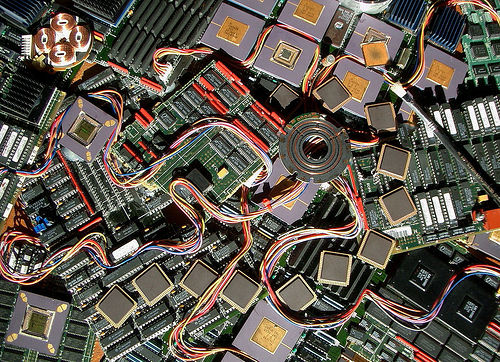
\includegraphics[width=.8\textwidth]{photos/siliconby-jurveston.jpg}\par
\textit{Picture by jurveston on Flickr.com}
\end{center}
\end{minipage}
\par \label{m38708*eip-586}\vspace{.5cm} 
      \noindent
   %   \hspace*{-30pt}
\includegraphics[width=0.5in]{col11305.imgs/pspencil2.png}   \raisebox{25mm}{   
   %   \begin{mdframed}[linewidth=4, leftmargin=40, rightmargin=40]  
      \begin{wex}{Metals, metalloids and non-metals 1}{\label{m38708*eip-77}
  \label{m38708*eip-252}
For each of the following substances state whether they are metals, metalloids or non-metals, using their position on the periodic table.
\label{m38708*eip-id1170734629720}
\begin{enumerate}[noitemsep, label=\textbf{\alph*}. ] 
            \leftskip=20pt\rightskip=\leftskip
\item Oxygen
\item Arsenic
\item Vanadium
\item Potassium
\end{enumerate}
  \par }
{\vspace{5pt}
%\label{m38708*eip-149}\noindent\textbf{Solution to Exercise }
%\label{m38708*eip-id1170750216596}\begin{enumerate}[noitemsep, label=\textbf{\alph*}. ] 
%            \leftskip=20pt\rightskip=\leftskip
\westep {Look at the periodic table} 
\begin{enumerate}[noitemsep, label=\textbf{\alph*}. ]
\item Oxygen is on the right of the zigzag line and so is a non-metal.
\item Arsenic is on the zigzag line and is a metalloid.
\item Vanadium is on the left of zigzag line and so is a metal.
\item Potassium is on the left of the zigzag line and so is a metal.\end{enumerate}
}
    \end{wex}
 %   \end{mdframed}
  %  }
%    \noindent
  \par
%            \label{m38708*eip-173}\vspace{.5cm} 
%      \noindent
%      \hspace*{-30pt}
\includegraphics[width=0.5in]{col11305.imgs/pspencil2.png}   \raisebox{25mm}{   
%      \begin{mdframed}[linewidth=4, leftmargin=40, rightmargin=40]  
      \begin{wex}{Metals, metalloids and non-metals 2}{\label{m38708*eip-757}
  \label{m38708*eip-25442}For each of the following substances state whether they are metals, metalloids or non-metals, using the information given.
\label{m38708*eip-id1170742635239}
\begin{enumerate}[noitemsep, label=\textbf{\alph*}. ] 
            \leftskip=20pt\rightskip=\leftskip
\item Aluminium in a cooking pot
\item Silicon in a computer chip
\item Plastic insulation around a wire
\item Silver jewellery\end{enumerate}
  \par }
{\vspace{5pt}
%\label{m38708*eip-1455}\noindent\textbf{Solution to Exercise }
%\label{m38708*eip-id1170755988427}\begin{enumerate}[noitemsep, label=\textbf{\alph*}. ] 
 %           \leftskip=20pt\rightskip=\leftskip
\westep{Use what you know} \begin{enumerate}[noitemsep, label=\textbf{\alph*}. ]
\item A cooking pot needs to be able to conduct heat and so the aluminium used must be a metal.
\item Computer chips rely on semi-conductors and all metalloids are semiconductors. So silicon is a metalloid.
\item The plastic around the wire must be insulating to current and so is a non-metal.
\item Silver in the jewellery is chosen for its malleability and shiny lustre. So silver is a metal.
\end{enumerate}}
    \end{wex}
%    \end{mdframed}
%    }
    \noindent
%   \label{m38708**end}
%          \section{Properties}
%     \nopagebreak
    \label{m38706*cid6}
            \section{Electrical conductors, semi-conductors and insulators}
            \nopagebreak
            \label{m38706} $ \hspace{-5pt}\begin{array}{cccccccccccc}   
\includegraphics[width=0.75cm]{col11305.imgs/summary_simulation.png} &   
\includegraphics[width=0.75cm]{col11305.imgs/summary_video.png} &   \end{array} $ \hspace{2 pt}\raisebox{-5 pt}{} {(section shortcode: P10012 )} \par 

            \label{m38706*id66058}An \textbf{electrical conductor} is a substance that allows an electrical current to pass through it. Electrical conductors are usually metals. \textsl{Copper} is one of the best electrical conductors, and this is why it is used to make conducting wire. In reality, \textsl{silver} actually has an even higher electrical conductivity than copper, but because silver is so expensive, it is not practical to use it for electrical wiring because such large amounts are needed. In the overhead power lines that we see above us, \textsl{aluminium} is used. The aluminium usually surrounds a steel core which adds tensile strength to the metal so that it doesn't break when it is stretched across distances. Occasionally gold is used to make wire, not because it is a particularly good conductor, but because it is very resistant to surface corrosion. \textsl{Corrosion} is when a material starts to deteriorate at the surface because of its reactions with the surroundings, for example oxygen and water in the air.\par 
      \label{m38706*id66098}An \textbf{insulator} is a non-conducting material that does not carry any charge. Examples of insulators would be plastic and wood. Do you understand now why electrical wires are normally covered with plastic insulation? \textbf{Semi-conductors} behave like insulators when they are cold, and like conductors when they are hot. The elements silicon and germanium are examples of semi-conductors.\par 
\Definition
%	  \begin{tabular*}{15 cm}{m{15 mm}m{}}
%	\hspace*{-50pt}  
\includegraphics[width=0.5in]{col11305.imgs/psflag2.png}   & \Definition{   \label{id2409398}\textbf{ 
{Conductors} 
%}} { \label{m38706*meaningfhsst!!!underscore!!!id354}
%      \label{m38706*id66124}
{A conductor allows the easy movement or flow of something such as heat or electrical charge through it.  \par 
       } 
\Definition{Insulators}
{Insulators are the opposite to conductors because they \textsl{inhibit} or reduce the flow of heat, electrical charge, sound etc through them. \par}

%      \end{tabular*}
%      \end{definition}
\label{m38706*id0522}Think about the materials around you. Are they electrical conductors or not? Why are different materials used? Think about the use of semiconductors in electronics? Can you think of why they are used there?\par 
\label{m38706*secfhsst!!!underscore!!!id357}
            \begin{i_experiment}{Electrical conductivity}{
            \nopagebreak
            \label{m38706*id66151}\noindent{}\textbf{Aim:}
        \newline
To investigate the electrical conductivity of a number of substances\par 
      \label{m38706*id66166}\noindent{}\textbf{Apparatus:}
        \newline
      \label{m38706*id66175}\begin{itemize}[noitemsep]
            \label{m38706*uid95}\item two or three cells
\label{m38706*uid96}\item light bulb
\label{m38706*uid97}\item crocodile clips
\label{m38706*uid98}\item wire leads
\label{m38706*uid99}\item a selection of test substances (e.g. a piece of plastic, aluminium can, metal pencil sharpener, magnet, wood, chalk).
\end{itemize}
        \par 
      \label{m38706*id66241}
    \setcounter{subfigure}{0}
	\begin{figure}[H] % horizontal\label{m38706*id66244}
    \begin{center}
\begin{pspicture}(0,-0.6)(5,6)
\SpecialCoor
%\psgrid[gridcolor=lightgray]
\pnode(0,0){A}
\pnode(0,5){B}
\pnode(5,5){C}
\pnode(5,0){D}
\pnode(3.5,0){E}
\pnode(1.5,0){F}
\rput{90}{\lamp(A)(B){light bulb}}
\battery(B)(C){battery}
\psline(C)(D)
\psline[arrowsize=10pt,arrowinset=0,arrowlength=2.5]{->}(D)(E)
\psframe(1.5,-0.5)(3.5,0.5)
\uput[u](2.5,0.5){test substance}
\rput(2.5,0){X}
\psline(4,0)(4,-0.4)(4.6,-0.4)
\uput[r](4.6,-0.4){crocodile clip}
\psline[arrowsize=10pt,arrowinset=0,arrowlength=2.5]{<-}(F)(A)
\end{pspicture}
    \end{center}
 \end{figure}       
      \par 
      \label{m38706*id66251}\noindent{}\textbf{Method:}
        \newline
      \label{m38706*id66260}\begin{enumerate}[noitemsep, label=\textbf{\arabic*}. ] 
            \label{m38706*uid100}\item Set up the circuit as shown above, so that the test substance is held between the two crocodile clips. The wire leads should be connected to the cells and the light bulb should also be connected into the circuit.
\label{m38706*uid101}\item Place the test substances one by one between the crocodile clips and see what happens to the light bulb.
\end{enumerate}
        \par 
      \label{m38706*id66291}\noindent{}\textbf{Results:}
        \newline
      Record your results in the table below:
    % \textbf{m38706*id66304}\par
          \begin{table}[H]
    % \begin{table}[H]
    % \\ '' '0'
        \begin{center}
      \label{m38706*id66304}
    \noindent
    \tabletail{%
        \hline
        \multicolumn{4}{|p{\mytableboxwidth}|}{\raggedleft \small \sl continued on next page}\\
        \hline
      }
      \tablelasttail{}
      \begin{xtabular}[t]{|l|l|l|l|}\hline
                \textbf{Test substance}
               &
                \textbf{Metal/non-metal}
               &
                \textbf{Does the light bulb glow?}
               &
                \textbf{Conductor or insulator}
              % make-rowspan-placeholders
     \tabularnewline\cline{1-1}\cline{2-2}\cline{3-3}\cline{4-4}
      %--------------------------------------------------------------------
         &
         &
         &
        % make-rowspan-placeholders
     \tabularnewline\cline{1-1}\cline{2-2}\cline{3-3}\cline{4-4}
      %--------------------------------------------------------------------
         &
         &
         &
        % make-rowspan-placeholders
     \tabularnewline\cline{1-1}\cline{2-2}\cline{3-3}\cline{4-4}
      %--------------------------------------------------------------------
         &
         &
         &
        % make-rowspan-placeholders
     \tabularnewline\cline{1-1}\cline{2-2}\cline{3-3}\cline{4-4}
      %--------------------------------------------------------------------
         &
         &
         &
        % make-rowspan-placeholders
     \tabularnewline\cline{1-1}\cline{2-2}\cline{3-3}\cline{4-4}
      %--------------------------------------------------------------------
    \end{xtabular}
      \end{center}
%    \begin{center}{\small\bfseries Table 1.3}\end{center}
%    \begin{caption}{\small\bfseries Table 1.3}\end{caption}
\end{table}
    \par
  \par 
      \label{m38706*id66494}\noindent{}\textbf{Conclusions:}
        \newline
  In the substances that were tested, the metals were able to conduct electricity and the non-metals were not. Metals are good electrical conductors and non-metals are not.\par }
            \end{i_experiment}
\label{m38706*eip-316}The following simulation allows you to work through the above activity. For this simulation use the grab bag option to get materials to test. Set up the circuit as described in the activity.
    \setcounter{subfigure}{0}
	\begin{figure}[H] % horizontal\label{m38806*transverse-waves}
    \textnormal{Phet simulation for Electrical conductivity}\vspace{.1in} \nopagebreak
  \label{m38806*phet!!!underscore!!!sim}\label{m38806*phet-simulation}
            \raisebox{-5 pt}{ 
\includegraphics[width=0.5cm]{col11305.imgs/summary_www.png}} { (Simulation:  lbK )}
      \vspace{2pt}
    \vspace{.1in}
 \end{figure}    
        \par 
    \label{m38706*cid7}
            \section{Thermal Conductors and Insulators}
            \nopagebreak
      \label{m38706*id66527}A \textbf{thermal conductor} is a material that allows energy in the form of heat, to be transferred within the material, without any movement of the material itself. An easy way to understand this concept is through a simple demonstration.\par 
\label{m38706*secfhsst!!!underscore!!!id453}
            \begin{gexperiment}{Demonstration:Thermal conductivity}{
            \nopagebreak
            \label{m38706*id66568}\noindent{}\textbf{Aim: }\newline
    To demonstrate the ability of different substances to conduct heat.\par 
      \label{m38706*id66588}\noindent{}\textbf{Apparatus: }\newline
    You will need two cups (made from the same material e.g. plastic); a metal spoon and a plastic spoon.\par 
	\begin{figure}[H] % horizontal\label{m38706*id66244}
    \begin{center}
\scalebox{0.6}{
\begin{pspicture}(-5,-5)(5,5)
\psset{unit=1cm}
\uput[r](-3,1){\large{boiling water}}
\psline[linewidth=0.04]{->}(-0.3,1)(0.5,1)
\uput[r](-3,3){\large{plastic spoon}}
\psline[linewidth=0.04]{->}(-0.25,3)(0.2,3)
\psline[linewidth=0.1](1.95,0)(0.25,3.2)
\pstTubeEssais[glassType=becher]
\uput[r](3.5,1){\large{boiling water}}
\psline[linewidth=0.04]{->}(3.55,1)(2.6,1)
\uput[r](3.5,3){\large{metal spoon}}
\psline[linewidth=0.04]{->}(3.55,3)(3,3)
\psline[linewidth=0.1](0.95,0)(3,3.2)
\pstTubeEssais[glassType=becher]
\end{pspicture}}
    \end{center}
 \end{figure} 
      \label{m38706*id66592}\noindent{}\textbf{Method: }
      \label{m38706*id66609}\begin{itemize}[noitemsep]
            \label{m38706*uid102}\item Pour boiling water into the two cups so that they are about half full.
\label{m38706*uid103}\item At the same time, place a metal spoon into one cup and a plastic spoon in the other.
\label{m38706*uid104}\item Note which spoon heats up more quickly
\end{itemize}
        \par 
\label{m38706*eip-270}
%\begin{tabular}{cc}
%	\hspace*{-50pt}\raisebox{-8 mm}{\hspace{-0.2in}
\includegraphics[width=0.5in]{col11305.imgs/pstip2.png} } & 
%	\begin{minipage}{0.85\textwidth}
%	\begin{note}
      \Warning{Be careful when working with boiling water and when you touch the spoons as you can easily burn yourself.}
%	\end{note}
%	\end{minipage}
%	\end{tabular}
	\par
      \label{m38706*id66666}\noindent{}\textbf{Results: }\newline
    The metal spoon heats up faster than the plastic spoon. In other words, the metal conducts heat well, but the plastic does not.\par 
\label{m38706*id66687}\noindent{}\textbf{Conclusion: }Metal is a good thermal conductor, while plastic is a poor thermal conductor. This explains why cooking pots are metal, but their handles are often plastic or wooden. The pot itself must be metal so that heat from the cooking surface can heat up the pot to cook the food inside it, but the handle is made from a poor thermal conductor so that the heat does not burn the hand of the person who is cooking.}
%This needs a diagram
 \par 
      \label{m38706*id66699}An \textbf{insulator} is a material that does not allow a transfer of electricity or energy. Materials that are poor thermal conductors can also be described as being good thermal insulators.\par 
% \label{m38706*notfhsst!!!underscore!!!id490}
% \begin{tabular}{cc}
% 	\hspace*{-50pt}\raisebox{-8 mm}{\hspace{-0.2in}
\includegraphics[width=0.75in]{col11305.imgs/psfact2.png} } & 
% 	\begin{minipage}{0.85\textwidth}
% 	\begin{note}
%       {note: }Water is a better thermal conductor than air and conducts heat away from the body about 20 times more efficiently than air. A person who is not wearing a wetsuit, will lose heat very quickly to the water around them and can be vulnerable to hypothermia (this is when the body temperature drops very low). Wetsuits help to preserve body heat by trapping a layer of water against the skin. This water is then warmed by body heat and acts as an insulator. Wetsuits are made out of closed-cell, foam neoprene. Neoprene is a synthetic rubber that contains small bubbles of nitrogen gas when made for use as wetsuit material. Nitrogen gas has very low thermal conductivity, so it does not allow heat from the body (or the water trapped between the body and the wetsuit) to be lost to the water outside of the wetsuit. In this way a person in a wetsuit is able to keep their body temperature much higher than they would otherwise.
% 	\end{note}
% 	\end{minipage}
% 	\end{tabular}
	\par
\label{m38706*secfhsst!!!underscore!!!id492}
            \begin{gexperiment}{Investigation : A closer look at thermal conductivity}
{            \nopagebreak
      \label{m38706*id66744}Look at the table below, which shows the thermal conductivity of a number of different materials, and then answer the questions that follow. The higher the number in the second column, the better the material is at conducting heat (i.e. it is a good thermal conductor). Remember that a material that conducts heat efficiently, will also lose heat more quickly than an insulating material.\par 
    % \textbf{m38706*id66753}\par
          \begin{table}[H]
    % \begin{table}[H]
    % \\ '' '0'
        \begin{center}
      \label{m38706*id66753}
    \noindent
      \begin{tabular}{|l|l|}\hline
\textbf{Material} & \textbf{Thermal Conductivity} \\ 
                 &  \textbf{($\mathrm{W}\ensuremath{\cdot}\mathrm{m}{}^{-1}\ensuremath{\cdot}\mathrm{K}{}^{-1}$) } \\ \hline
Silver & 429 \\ \hline
Stainless steel & 16 \\ \hline
Standard glass & 1.05 \\ \hline
Concrete & 0.9 - 2 \\ \hline
Red brick & 0.69 \\ \hline
Water & 0.58 \\ \hline
Snow & 0.25 - 0.5 \\ \hline
Wood & 0.04 - 0.12 \\ \hline
Polystyrene & 0.03 \\ \hline
Air & 0.024 \\ \hline
    \end{tabular}
      \end{center}
%    \begin{center}{\small\bfseries Table 1.4}\end{center}
%    \begin{caption}{\small\bfseries Table 1.4}\end{caption}
\end{table}
    \par
      \label{m38706*id67009}Use this information to answer the following questions:\par 
      \label{m38706*id67013}\begin{enumerate}[noitemsep, label=\textbf{\arabic*}. ] 
            \label{m38706*uid105}\item Name two materials that are good thermal conductors.
\label{m38706*uid106}\item Name two materials that are good insulators.
\label{m38706*uid107}\item Explain why:
\label{m38706*id67053}\begin{enumerate}[noitemsep, label=\textbf{\alph*}. ] 
            \label{m38706*uid108}\item cooler boxes are often made of polystyrene
\label{m38706*uid109}\item homes that are made from wood need less internal heating during the winter months.
\label{m38706*uid110}\item igloos (homes made from snow) are so good at maintaining warm temperatures, even in freezing conditions.
\end{enumerate}
        \end{enumerate}}
\end{gexperiment}
\label{m38706*notfhsst!!!underscore!!!id564}
%\begin{tabular}{cc}
%	\hspace*{-50pt}\raisebox{-8 mm}{\hspace{-0.2in}
\includegraphics[width=0.75in]{col11305.imgs/psfact2.png} } & 
%	\begin{minipage}{0.85\textwidth}
%	\begin{note}
      \IFact{It is a known fact that well-insulated buildings need less energy for heating than do buildings that have no insulation. Two building materials that are being used more and more worldwide, are \textbf{mineral wool} and \textbf{polystyrene}. Mineral wool is a good insulator because it holds air still in the matrix of the wool so that heat is not lost. Since air is a poor conductor and a good insulator, this helps to keep energy within the building. Polystyrene is also a good insulator and is able to keep cool things cool and hot things hot. It has the added advantage of being resistant to moisture, mould and mildew.}
%	\end{note}
%	\end{minipage}
%	\end{tabular}
	\par
      \label{m38706*id67129}Remember that concepts such as conductivity and insulation are not only relevant in the building, industrial and home environments. Think for example of the layer of blubber or fat that is found in some animals. In very cold environments, fat and blubber not only provide protection, but also act as an insulator to help the animal keep its body temperature at the right level. This is known as \textsl{thermoregulation}.\par 
    \label{m38706*cid8}
            \section{Magnetic and Non-magnetic Materials}
            \nopagebreak
      \label{m38706*id67151}We have now looked at a number of ways in which matter can be grouped, such as into metals, semi-metals and non-metals; electrical conductors and insulators, and thermal conductors and insulators. One way in which we can further group metals, is to divide them into those that are \textbf{magnetic} and those that are \textbf{non-magnetic.}\par 
\par
%             \label{m38706*fhsst!!!underscore!!!id570}\begin{definition}
% 	  \begin{tabular*}{15 cm}{m{15 mm}m{}}
% 	\hspace*{-50pt}  
\includegraphics[width=0.5in]{col11305.imgs/psflag2.png}   & 
\Definition{   \label{id2410309} { Magnetism }} { \label{m38706*meaningfhsst!!!underscore!!!id570}
      \label{m38706*id67174}Magnetism is a force that certain kinds of objects, which are called `magnetic' objects, can exert on each other without physically touching. A magnetic object is surrounded by a magnetic `field' that gets weaker as one moves further away from the object. \par 
       } 
%       \end{tabular*}
%       \end{definition}
      \label{m38706*id67186}A metal is said to be \textbf{ferromagnetic} if it can be magnetised (i.e. made into a magnet). If you hold a magnet very close to a metal object, it may happen that its own electrical field will be induced and the object becomes magnetic. Some metals keep their magnetism for longer than others. Look at iron and steel for example. Iron loses its magnetism quite quickly if it is taken away from the magnet. Steel on the other hand will stay magnetic for a longer time. Steel is often used to make permanent magnets that can be used for a variety of purposes.\par 
      \label{m38706*id67200}Magnets are used to sort the metals in a scrap yard, in compasses to find direction, in the magnetic strips of video tapes and ATM cards where information must be stored, in computers and TV's, as well as in generators and electric motors.\par 
\label{m38706*secfhsst!!!underscore!!!id575}
            \begin{gexperiment}{Investigation : Magnetism}{
            \nopagebreak
      \label{m38706*id67220}You can test whether an object is magnetic or not by holding another magnet close to it. If the object is attracted to the magnet, then it too is magnetic.\par 
      \label{m38706*id67227}Find five objects in your classroom or your home and test whether they are magnetic or not. Then complete the table below:\par 
    % \textbf{m38706*id67234}\par
          \begin{table}[H]
    % \begin{table}[H]
    % \\ '' '0'
        \begin{center}
      \label{m38706*id67234}
    \noindent
      \begin{tabular}{|l|l|}\hline
                \textbf{Object}
               &
                \textbf{Magnetic or non-magnetic} \\ \hline
         & \\ \hline
         & \\ \hline
         & \\ \hline
         & \\ \hline
         & \\ \hline
    \end{tabular}
      \end{center}
%     \begin{center}{\small\bfseries Table 1.5}\end{center}
%     \begin{caption}{\small\bfseries Table 1.5}\end{caption}
\end{table}}
\end{gexperiment}
    \par
\label{m38706*secfhsst!!!underscore!!!id616}
            \begin{groupdiscussion}{Group Discussion : Properties of materials}{
            \nopagebreak
      \label{m38706*id67392}In groups of 4-5, discuss how our knowledge of the properties of materials has allowed society to:\par 
      \label{m38706*id67398}\begin{itemize}[noitemsep]
            \label{m38706*uid111}\item develop advanced computer technology
\label{m38706*uid112}\item provide homes with electricity
\label{m38706*uid113}\item find ways to conserve energy
\end{itemize}
\end{groupdiscussion}
\label{m38706*eip-968}The following presentation provides a summary of the classification of matter.
    \setcounter{subfigure}{0}
	\begin{figure}[H] % horizontal\label{m38706*slidesharefigure}
    \label{m38706*slidesharemedia}\label{m38706*slideshareflash}\raisebox{-5 pt}{ 
\includegraphics[width=0.5cm]{col11305.imgs/summary_www.png}} { (Presentation:  P10013 )}
      \vspace{2pt}
    \vspace{.1in}
 \end{figure}       \par}
\end{discussion} \label{m38706*cid9}
            \section{Summary}
            \nopagebreak
      \label{m38706*id67458}\begin{itemize}[noitemsep]
            \label{m38706*uid114}\item All the objects and substances that we see in the world are made of \textbf{matter}.
\label{m38706*uid115}\item This matter can be classified according to whether it is a \textbf{mixture} or a \textbf{pure substance}.
\label{m38706*uid116}\item A \textbf{mixture} is a combination of one or more substances that are not chemically bonded to each other. Examples of mixtures are air (a mixture of different gases) and blood (a mixture of cells, platelets and plasma).
\label{m38706*uid117}\item The main \textbf{characteristics} of mixtures are that the substances that make them up are not in a fixed ratio, they keep their individual properties and they can be separated from each other using mechanical means.
\label{m38706*uid118}\item A \textbf{heterogeneous mixture} is non-uniform and the different parts of the mixture can be seen. An example would be a mixture of sand and water.
\label{m38706*uid119}\item A \textbf{homogeneous mixture} is uniform, and the different components of the mixture can't be seen. An example would be a salt solution. A salt solution is a mixture of salt and water. The salt dissolves in the water, meaning that you can't see the individual salt particles. They are interspersed between the water molecules. Another example is a metal \textbf{alloy} such as steel.
\label{m38706*uid120}\item Mixtures can be \textbf{separated} using a number of methods such as filtration, heating, evaporation, centrifugation and dialysis.
\label{m38706*uid121}\item Pure substances can be further divided into \textbf{elements} and \textbf{compounds}.
\label{m38706*uid122}\item An \textbf{element} is a substance that can't be broken down into simpler substances through chemical means.
\label{m38706*uid123}\item All the elements are recorded in the \textbf{Periodic Table of the Elements}. Each element has its own chemical symbol. Examples are iron ($\mathrm{Fe}$), sulphur ($\mathrm{S}$), calcium ($\mathrm{Ca}$), magnesium ($\mathrm{Mg}$) and fluorine ($\mathrm{F}$).
\label{m38706*uid124}\item A \textbf{compound} is a substance that is made up of two or more elements that are chemically bonded to each other in a fixed ratio. Examples of compounds are sodium chloride ($\mathrm{NaCl}$), iron sulphide ($\mathrm{FeS}$), calcium carbonate (${\mathrm{CaCO}}_{3}$) and water (${\mathrm{H}}_{2}\mathrm{O}$).
\label{m38706*uid125}\item When \textbf{naming compounds} and writing their \textbf{chemical formula}, it is important to know the elements that are in the compound, how many atoms of each of these elements will combine in the compound and where the elements are in the Periodic Table. A number of rules can then be followed to name the compound.
\label{m38706*uid126}\item Another way of classifying matter is into \textbf{metals} (e.g. iron, gold, copper), \textbf{semi-metals} (e.g. silicon and germanium) and \textbf{non-metals} (e.g. sulphur, phosphorus and nitrogen).
\label{m38706*uid127}\item \textbf{Metals} are good electrical and thermal conductors, they have a shiny lustre, they are malleable and ductile, and they have a high melting point. These properties make metals very useful in electrical wires, cooking utensils, jewellery and many other applications.
\label{m38706*uid128}\item A further way of classifying matter is into \textbf{electrical conductors}, \textbf{semi-conductors} and \textbf{insulators}.
\label{m38706*uid129}\item An \textbf{electrical conductor} allows an electrical current to pass through it. Most metals are good electrical conductors.
\label{m38706*uid130}\item An \textbf{electrical insulator} is not able to carry an electrical current. Examples are plastic, wood, cotton material and ceramic.
\label{m38706*uid131}\item Materials may also be classified as \textbf{thermal conductors} or \textbf{thermal insulators} depending on whether or not they are able to conduct heat.
\label{m38706*uid132}\item Materials may also be either \textbf{magnetic} or \textbf{non-magnetic}.
\end{itemize}
\label{m38706*secfhsst!!!underscore!!!id672}
            \begin{eocexercises}{Classification of matter }{
            \nopagebreak
      \label{m38706*id67920}\begin{enumerate}[noitemsep, label=\textbf{\arabic*}. ] 
            \label{m38706*uid133}\item For each of the following \textbf{multiple choice} questions, choose \textsl{one} correct answer from the list provided.
\label{m38706*id67947}\begin{enumerate}[noitemsep, label=\textbf{\alph*}. ] 
            \label{m38706*uid134}\item Which of the following can be classified as a mixture:
\label{m38706*id67963}\begin{enumerate}[noitemsep, label=\textbf{\alph*}. ] 
            \label{m38706*uid135}\item sugar
\label{m38706*uid136}\item table salt
\label{m38706*uid137}\item air
\label{m38706*uid138}\item iron
\end{enumerate}
                \label{m38706*uid139}\item An element can be defined as:
\label{m38706*id68029}\begin{enumerate}[noitemsep, label=\textbf{\alph*}. ] 
            \label{m38706*uid140}\item A substance that cannot be separated into two or more substances by ordinary chemical (or physical) means
\label{m38706*uid141}\item A substance with constant composition
\label{m38706*uid142}\item A substance that contains two or more substances, in definite proportion by weight
\label{m38706*uid143}\item A uniform substance
\end{enumerate}
                \end{enumerate}
\label{m38706*uid144}\item Classify each of the following substances as an \textsl{element}, a \textsl{compound}, a \textsl{solution} (homogeneous mixture), or a \textsl{heterogeneous mixture}: salt, pure water, soil, salt water, pure air, carbon dioxide, gold and bronze.\newline
\label{m38706*uid145}\item Look at the table below. In the first column (A) is a list of substances. In the second column (B) is a description of the group that each of these substances belongs in. Match up the \textsl{substance} in Column A with the \textsl{description} in Column B.
    % \textbf{m38706*id68147}\par
          \begin{table}[H]
    % \begin{table}[H]
    % \\ 'id2880342' '1'
        \begin{center}
      \label{m38706*id68147}
      \begin{tabular}{|l|l|}\hline
\textbf{Column A} & \textbf{Column B} \\ \hline
iron & a compound containing 2 elements \\ \hline
H$_\text{2}$S & a heterogeneous mixture \\ \hline
sugar solution & a metal alloy \\ \hline
sand and stones & an element \\ \hline
steel & a homogeneous mixture \\ \hline
    \end{tabular}
      \end{center}
%     \begin{center}{\small\bfseries Table 1.6}\end{center}
%     \begin{caption}{\small\bfseries Table 1.6}\end{caption}
\end{table}
    \par
\label{m38706*uid146}\item You are given a test tube that contains a mixture of iron filings and sulphur. You are asked to weigh the amount of iron in the sample.
\label{m38706*id68262}\begin{enumerate}[noitemsep, label=\textbf{\alph*}. ] 
            \label{m38706*uid147}\item Suggest one method that you could use to separate the iron filings from the sulphur.
\label{m38706*uid148}\item What property of metals allows you to do this?
\end{enumerate}
\label{m38706*uid149}\item Given the following descriptions, write the chemical formula for each of the following substances:
\label{m38706*id68304}\begin{enumerate}[noitemsep, label=\textbf{\alph*}. ] 
            \label{m38706*uid150}\item silver metal
\label{m38706*uid151}\item a compound that contains only potassium and bromine
\label{m38706*uid152}\item a gas that contains the elements carbon and oxygen in a ratio of 1:2
\end{enumerate}
\label{m38706*uid153}\item Give the names of each of the following compounds:
\label{m38706*id68358}\begin{enumerate}[noitemsep, label=\textbf{\alph*}. ] 
            \label{m38706*uid154}\item $\mathrm{NaBr}$
\label{m38706*uid155}\item ${\mathrm{BaSO}}_{4}$\label{m38706*uid156}\item ${\mathrm{SO}}_{2}$ \end{enumerate}
\label{m38706*uid157}\item For each of the following materials, say what properties of the material make it important in carrying out its particular function.
\label{m38706*id68436}\begin{enumerate}[noitemsep, label=\textbf{\alph*}. ] 
            \label{m38706*uid158}\item \textbf{tar} on roads
\label{m38706*uid159}\item \textbf{iron} burglar bars
\label{m38706*uid160}\item \textbf{plastic} furniture
\label{m38706*uid161}\item \textbf{metal} jewellery
\label{m38706*uid162}\item \textbf{clay} for building
\label{m38706*uid163}\item \textbf{cotton} clothing
\end{enumerate}
\end{enumerate}
  \label{m38706**end}
  \label{09a7a4809656be0b739ee130746cd803**end}
\par \raisebox{-5 pt}{
\includegraphics[width=0.5cm]{col11305.imgs/summary_www.png}} Find the answers with the shortcodes:
 \par \begin{tabular}[h]{cccccc}
 (1.) ll6  &  (2.) llF  &  (3.) llG  &  (4.) ll7  &  (5.) llA  &  (6.) llo  &  (7.) lls  &  (8.) llH  & \end{tabular}}
\end{eocexercises}
